% Exemplo de dissertação do INF-UFG com texto em portugues formatado com LaTeX
\documentclass[relatorio]{inf-ufg}
% Opções da classe inf-ufg (ao usar mais de uma, separe por vírgulas)
%   [tese]         -> Tese de doutorado.
%   [dissertacao]  -> Dissertação de mestrado (padrão).
%   [monografia]   -> Monografia de especialização.
%   [relatorio]    -> Relatório final de graduação.
%   [abnt]         -> Usa o estilo "abnt-alf" de citação bibliográfica.
%   [nocolorlinks] -> Os links de navegação no texto ficam na cor preta.
%                     Use esta opção para gerar o arquivo para impressão
%                     da versão final do seu texto!!!

%----------------------------------------------------- INICIO DO DOCUMENTO %
\begin{document}

%------------------------------------------ AUTOR, TÍTULO E DATA DE DEFESA %
\autor{Murillo Rodrigues de Paula} % (José da Silva)
\autorR{Paula, Murillo Rodrigues de} % (da Silva, José)

\titulo{Implementação de uma biblioteca cliente HTTP/2 multiplataforma em Lua}
%\subtitulo{\textless Subtítulo do TRabalho\textgreater}

\cidade{Goiânia} % Nome da cidade em foi desenvolvido o trabalho
\dia{07} %
\mes{12} % Data da apresentação/defesa do trabalho
\ano{2018} % Formato numérico: \dia{01}, \mes{01} e \ano{2009}

%-------------------------------------------------------------- ORIENTADOR %
\orientador{Bruno Oliveira Silvestre}
\orientadorR{Silvestre, Bruno Oliveira}
% Use os comandos a seguir se for Orientadora e nao Orientador.
%\orientadora{\textless Nome da Orientadora\textgreater}
%\orientadoraR{\textless Nome Reverso da Orientadora\textgreater}

%\coorientador{\textless Nome do Co-orientador\textgreater}
%\coorientadorR{\textless Nome Reverso do Co-orientador\textgreater}
% Use os comandos a seguir se for Co-orientadora e nao Coorientador.
%\coorientadora{\textless Nome da Co-orientadora\textgreater}
%\coorientadoraR{\textless Nome Reverso da Co-orientadora\textgreater}

%-------------------------------------------------- INSTITUIÇÃO E PROGRAMA %
\universidade{Universidade Federal de Goiás} % {Universidade Federal de Goiás}
\uni{UFG}         % UFG
\unidade{Instituto de Informática} %Instituto de Informática
%\departamento{\textless Nome do Departamento\textgreater} %Unidades com mais de um depto.

%\universidadeco{\textless Nome da Universidade do Co-orientador\textgreater}
%\unico{\textless Sigla da Universidade do Co-orientador\textgreater}
%\unidadeco{\textless Nome da Unidade Acadêmica do Co-orientador\textgreater}

%\programa{\textless Nome do Programa de Pós-Graduação\textgreater} % Computação
\concentracao{Ciência da Computação}

%-------------------------------------------------- ELEMENTOS PRÉ-TEXTUAIS %
\capa    % Gera o modelo da capa externa do trabalho
\publica % Gera a autorização para publicação em formato eletrônico
\rosto   % Primeira folha interna do trabalho

\begin{figure}[hbt!]
 \centering
  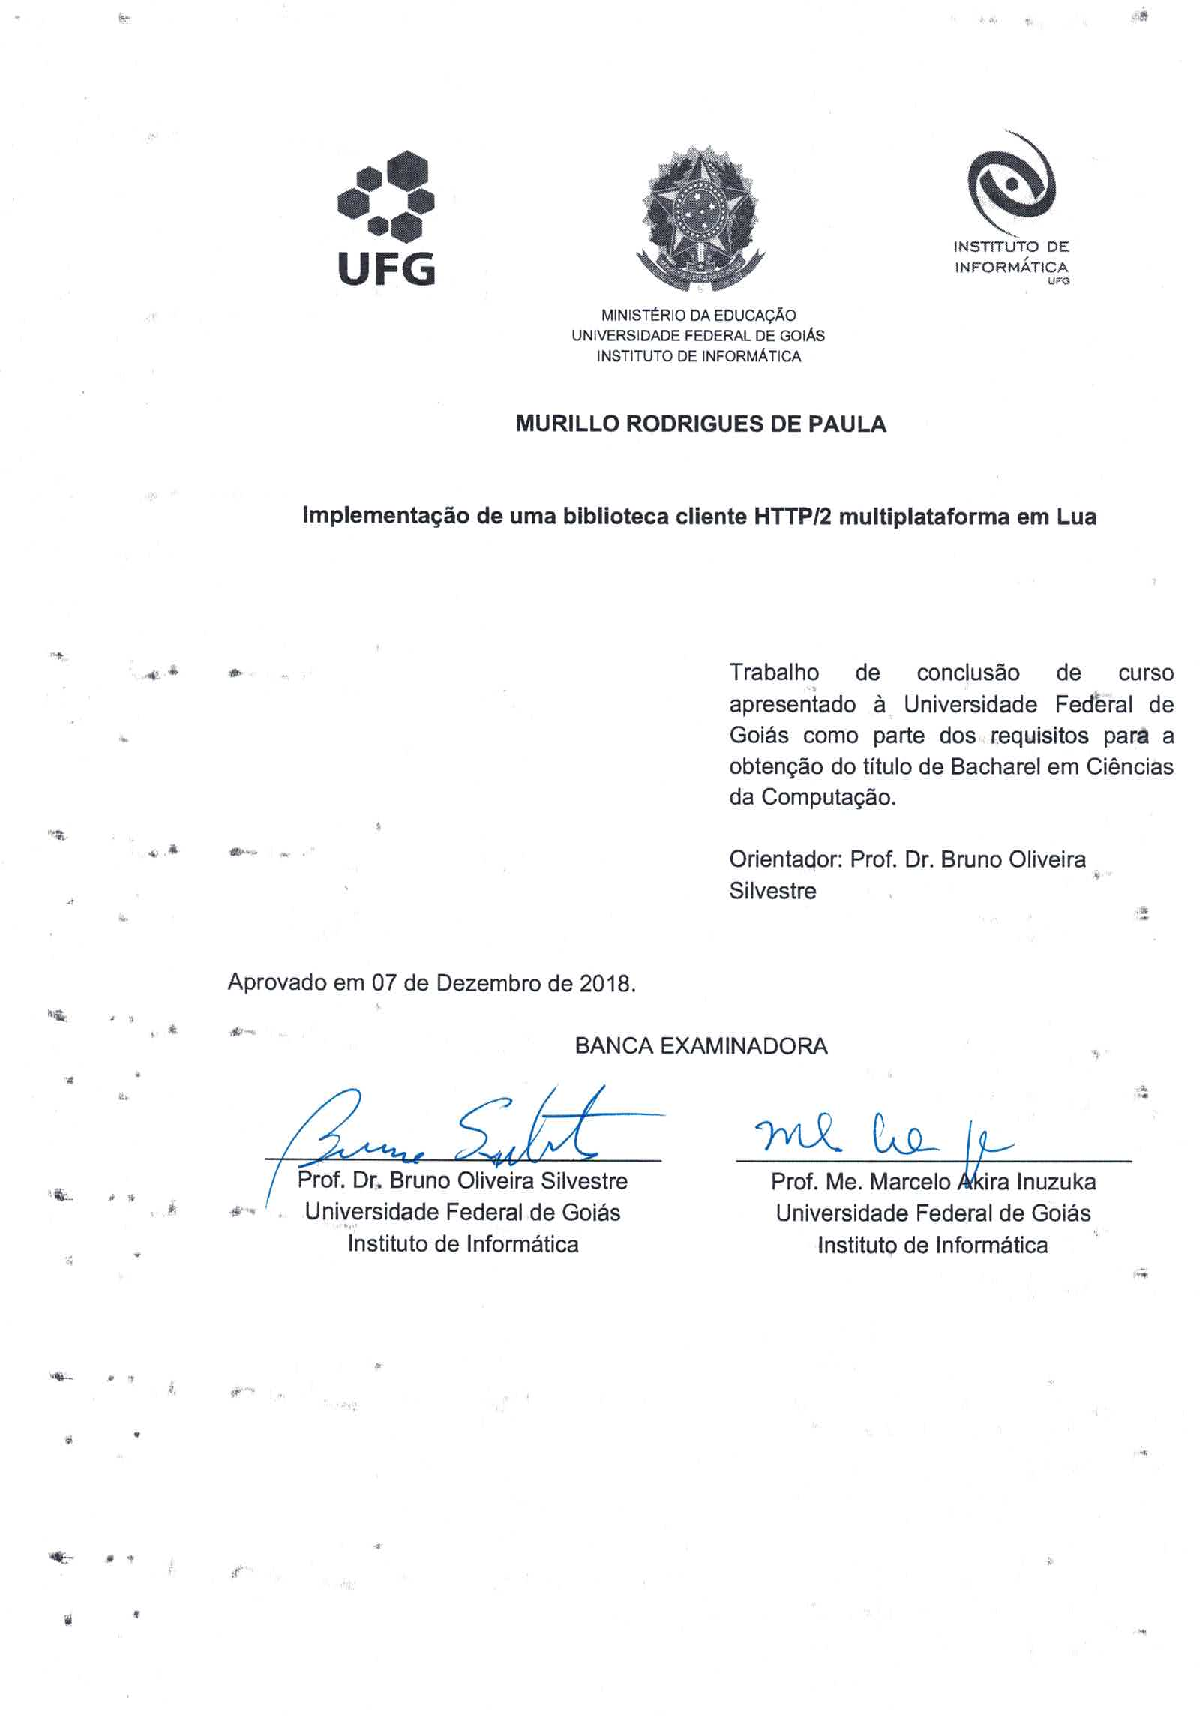
\includegraphics[width=\textwidth]{./aprov}
\end{figure}
\direitos{Graduando em Ciência da Computação na UFG - Universidade Federal de Goiás. Durante sua graduação, foi monitor da disciplina Linguagens de Programação no Instituto de Informática da UFG por um ano, realizou atividades de estágio pela Rede Nacional de Ensino e Pesquisa (RNP) por um ano e participou da Maratona de Programação ICPC por dois anos consecutivos.}

\begin{dedicatoria}
Dedico este trabalho à minha mãe e ao meu pai.
\end{dedicatoria}

\begin{agradecimentos}

Eu serei eternamente grato por todas as pessoas que de uma forma ou de outra me ajudaram na produção deste projeto. Primeiro, eu agradeço a Deus pela proteção e pela habilidade de poder estudar e trabalhar.

Ao Professor Bruno Silvestre, meu orientador. Enquanto meu orientador, professor e mentor, ele já me ensinou mais do que eu poderia escrever aqui. Ele vem me mostrado, por seu exemplo, como um bom cientista deveria ser e agir. Sem sua ajuda e apoio do começo ao fim, este projeto não seria possível.

Ao Professor Marcelo Akira, que conheci como orientador inicial do presente trabalho e hoje integra a Banca Examinadora. Obrigado pelas contribuições iniciais deste trabalho e por me ensinar a ter proatividade em projetos de software livre.

Ao apoio dos meus amigos, principalmente do Eduardo. Obrigado pela inspiração, pelas críticas, pelo aprendizado e pela agradável companhia durante a graduação.

À minha companheira Larissa, pelo amor e carinho.

Por fim, ninguém tem sido mais importante para mim nessa jornada do que os membros da minha família. Eu gostaria de agradecer especialmente aos meus pais, cujo o amor e o apoio incondicional durante toda a minha vida me possibilitaram lutar pelos meus sonhos.
\end{agradecimentos}


\epigrafe{Simple can be harder than complex: You have to work hard to get your thinking clean to make it simple. But it’s worth it in the end because once you get there, you can move mountains.}
{Steve Jobs}
{Entrevista com Business Week, 1998}
:
\chaves{Cliente HTTP/2, Linguagem Lua, Programação Orientada a Eventos.}

\begin{resumo} 
Bibliotecas clientes HTTP/2 propiciam a escrita de códigos de clientes HTTP/2 altamente genéricos, principalmente nas linguagens de programação de {\em scripting}. No entanto, apenas uma biblioteca cliente HTTP/2 está disponível para a linguagem Lua e ela não é multiplataforma, pois funciona apenas em sistemas operacionais derivados do UNIX. Isso limita a portabilidade de clientes HTTP/2 que utilizam essa biblioteca uma vez que Lua é uma linguagem muito portátil. Neste trabalho, implementamos uma biblioteca cliente HTTP/2 multiplataforma em Lua. Ela é capaz de oferecer suporte às principais funcionalidades do protocolo HTTP/2, incluindo multiplexação de fluxos em uma única conexão TCP e compressão de cabeçalhos com o protocolo HPACK. Também realizamos testes que comprovam a eficiência de um cliente HTTP/2 escrito em cima da biblioteca quando comparado com outros três clientes HTTP/2: um em C (nghttp), um em JavaScript (Node.js) e outro na biblioteca HTTP/2 atualmente disponível para Lua (lua-http).
\end{resumo}


\keys{HTTP/2 Client, Lua Language, Event-driven Programming}

\begin{abstract}{Implementation of a multi-platform HTTP/2 client library in Lua.}
HTTP/2 client libraries allow the writing of highly generic HTTP/2 client code, especially in {\em scripting} programming languages. However, only one HTTP/2 client library is available for the Lua language and it is not multiplatform, since it works only on UNIX-like operating systems. This limits the portability of HTTP/2 clients that use this library because Lua is a very portable language. In this work, a multi-platform HTTP/2 client library in Lua was developed. It is capable of supporting the main features of the HTTP/2 protocol, including stream multiplexing in a single TCP connection and header compression with the HPACK protocol. Tests were performed that prove the efficiency of an HTTP/2 client written on top of the library when compared with three other HTTP/2 clients: one in C (nghttp), one in JavaScript (Node.js) and another in the currently available HTTP/2 library for Lua (lua-http).
\end{abstract}


\tabelas[figcod]
%Opções:
%nada [] -> Gera apenas o sumário
%fig     -> Gera o sumário e a lista de figuras
%tab     -> Sumário e lista de tabelas
%alg     -> Sumário e lista de algoritmos
%cod     -> Sumário e lista de códigos de programas
%
% Pode-se usar qualquer combinação dessas opções.
% Por exemplo:
%  figtab       -> Sumário e listas de figuras e tabelas
%  figtabcod    -> Sumário e listas de figuras, tabelas e
%                  códigos de programas
%  figtabalg    -> Sumário e listas de figuras, tabelas e algoritmos
%  figtabalgcod -> Sumário e listas de figuras, tabelas, algoritmos e
%                  códigos de programas

%--------------------------------------------------------------- CAPÍTULOS %
\chapter{Introdução}
\label{cap:intro}

Redes de computadores revolucionaram o mundo da ciência da computação. A Internet pública, uma rede de computadores específica, já é uma parte indivisível da estrutura das sociedades modernas e a força motriz por trás do seu sucesso se deve aos avanços da Web e do {\em Hypertext Transfer Protocol} (HTTP). A Web é uma aplicação cliente-servidor que permite usuários obterem páginas Web de servidores sob demanda e seu principal protocolo é o HTTP, um protocolo da camada de aplicação sem estado de requisição\slash resposta.

Apesar do sucesso da Web e do HTTP, requisitar páginas Web é uma tarefa cada vez mais intensiva em recursos de rede. Com o advento das aplicações Web, do número de usuários, da velocidade dos enlaces e da capacidade da rede como um todo, a adição de mais recursos como JavaScript, CSS, imagens e fontes às páginas Web aumentaram substancialmente e atualmente essa prática é considerada aceitável.

Nos últimos sete anos e seis meses, o tamanho (em kilobytes) de todos os recursos de um página Web requisitado por um computador pessoal aumentou em aproximadamente três vezes e aqueles requisitados por um dispositivo móvel aumentou em aproximadamente nove vezes \cite{HTTPArchive}. Transportar eficientemente todos esses recursos na rede é uma tarefa cada vez mais difícil.

Uma das causas dessa dificuldade está relacionada ao modo como o HTTP utiliza o protocolo da camada de transporte TCP: cada requisição por uma página Web usa uma conexão TCP separada. Com muitas requisições sendo enviadas, o aumento do número de conexões TCP gera uma monopolização dos recursos de rede. A outra causa está presente nas próprias mensagens HTTP: cada mensagem é enviada em texto simples na conexão TCP, contendo muitos cabeçalhos repetitivos e extensos.

Para resolver ambos esses problemas, uma nova versão do protocolo HTTP foi padronizada, denominada {\em Hypertext Transfer Protocol version 2} (HTTP/2) \cite{BelsheRFC7540}. Hoje, 46.5\% dos 1 milhão de sites mais acessados do mundo recebem requisições HTTP/2 \cite{HTTPArchive}. Nos navegadores, o HTTP/2 é suportado pelas últimas versões do Google Chrome, Mozilla Firefox, Microsoft Edge, Opera e Safari.

Além dos navegadores, requisições também são feitas por clientes HTTP/2 simples, implementados em uma linguagem de programação específica. Entre essas linguagens, destacam-se as linguagens dinâmicas. Geralmente, essas linguagens oferecem bibliotecas HTTP/2 reusáveis para a implementação de clientes que fazem as requisições para os servidores.

Usar bibliotecas promove mais modularidade aos códigos das aplicações e mais reusabilidade de código aos programadores, além de permitirem a escrita de códigos altamente genéricos. Com isso, clientes HTTP/2 podem ser implementados de modo independente desde que uma API ({\em Application Programming Interface}) bem definida seja fornecida pela biblioteca.

Entre as linguagens dinâmicas, a linguagem Lua \cite{Ierusalimschy2016PiL} tem se destacado não só pela flexibilidade em criar bibliotecas, mas também pela sua alta eficiência. Essa combinação a torna uma linguagem interessante para implementar o lado cliente do HTTP/2, visto que esse protocolo demanda eficiência por parte das implementações para que seus benefícios de desempenho às aplicações sejam mais bem aproveitados.

Lua também foi criada com portabilidade em mente porque foi implementada em ANSI (ISO) C e é pequena em tamanho. A biblioteca HTTP/2 atual \cite{DaurminatorLuaHTTP} disponível para Lua não segue esse objetivo porque ela só pode ser usada em sistemas operacionais derivados do UNIX e portanto não é uma biblioteca portátil multiplataforma. Ela é uma biblioteca externa e não faz parte do conjunto de bibliotecas padrões de Lua.

O propósito deste trabalho é apresentar uma implementação de uma biblioteca cliente HTTP/2 multiplataforma escrita em Lua. O intuito é fornecer suporte HTTP/2 para que aplicações Web escritas em Lua aproveitem os benefícios de desempenho trazidos por esse protocolo. Para isso, foi implementado uma biblioteca cliente capaz de prover uma API simples de um cliente HTTP/2 que pode user utilizada em qualquer aplicação Web escrita em Lua 5.3.

Testes de carga ({\em benchmarks}) foram feitos com o objetivo de comparar o desempenho da implementação. Comparamos um cliente escrito em cima da biblioteca criada com outros três clientes HTTP/2: um em C (nghttp), um em JavaScript (Node.js) e outro na biblioteca HTTP/2 atualmente disponível para Lua (lua-http). Pelos resultados obtidos, o cliente escrito na biblioteca HTTP/2 deste trabalho obteve desempenho igual ou superior em relação ao desempenho dos demais clientes, demonstrando assim sua eficiência.

A estrutura e a organização deste trabalho foram delineadas da seguinte forma: o Capítulo \ref{cap:theory} descreve as ferramentas conceituais do protocolo HTTP/2 e da linguagem Lua que viabilizaram a escrita da implementação; o Capítulo \ref{cap:implementation} apresenta a implementação, incluindo as decisões de projeto tomadas para orientar seu desenvolvimento e os problemas resolvidos; o Capítulo \ref{cap:results} apresenta os testes e comparações realizadas para comprovar a eficiência da implementação da biblioteca e o Capítulo \ref{cap:conclusion} apresenta as considerações finais sobre este trabalho.
\chapter{Fundamentos Teóricos}
\label{cap:theory}

Este capítulo apresentará uma visão geral dos fundamentos teóricos que permitiram a implementação da biblioteca cliente HTTP/2 em Lua. Conceituar o HTTP/2 e a linguagem Lua é de suma importância para sustentar as ideias da implementação. Para isso, o capítulo foi organizado em duas seções: uma seção dedicada à descrição do protocolo HTTP/2 e outra à linguagem Lua. Tanto o HTTP/2 quanto Lua são assuntos naturalmente extensos e portanto cada seção consiste de um breve resumo de conceitos que foram pertinentes à escrita da implementação.

A seção \ref{sec:http2} apresenta uma breve história do HTTP/2 e a natureza dos problemas de desempenho presentes no HTTP, destacando o escopo desses problemas, como eles se manifestam e como estudos passados tentaram resolvê-los. Depois, um breve resumo do protocolo HTTP/2 é apresentado. A completa definição do HTTP/2 é um produto dos RFCs 7540 \cite{BelsheRFC7540} e 7541 \cite{BelsheRFC7541} e podem ser consultados para informações mais detalhadas do protocolo.

A seção \ref{sec:lua} apresenta as principais características da linguagem de programação Lua, juntamente com as bibliotecas escritas em Lua que permitiram uma implementação compatível com a natureza de um cliente HTTP/2. Como a implementação da biblioteca foi feita em Lua, essa seção destaca os principais paradigmas e construções da linguagem que viabilizaram a escrita da biblioteca. Todos os aspectos da linguagem Lua são cobertos pelo livro Programming in Lua \cite{Ierusalimschy2016PiL}.

%% - - - - - - - - - - - - - - - - - - - - - - - - - - - - - - - - - - -
\section{HTTP/2}
\label{sec:http2}

O {\em Hypertext Transfer Protocol version 2} (HTTP/2) é um protocolo da camada de aplicação sem estado de requisição/resposta para sistemas de informação hipertextos, distribuídos e colaborativos definido pelos RFCs 7540 \cite{BelsheRFC7540} e 7541 \cite{BelsheRFC7541}. O RFC 7540 especifica uma nova sintaxe para o HTTP/2, mas não altera a semântica já existente do HTTP/1.1 e o RFC 7541 define um formato de compressão para campos de cabeçalhos HTTP/2.

Um dos propósitos pelo qual a especificação do HTTP/2 foi criada é o de proporcionar um melhor desempenho às aplicações Web ao permitir que clientes e servidores HTTP/2 façam um uso mais eficiente da conexão TCP \cite{Brylinski:2017:OH:3018896.3065841}, onde toda conexão é persistente e as requisições podem ser feitas de forma concorrente. No HTTP/1.1, clientes e servidores têm a opção de usar conexões persistentes ou não persistentes. Porém, quando conexões persistentes são usadas no HTTP/1.1, cada requisição é feita de forma sequencial, ou seja, requisições devem esperar por cada resposta do servidor.

Para que as requisições não precisem esperar por cada resposta, o HTTP/1.1 permitiu paralelismo ({\em pipelining}) de requisições, mas uma requisição que necessita de um processamento significativo no lado do servidor pode resultar em uma resposta grande e lenta, podendo bloquear outras requisições. Esse problema é conhecido como bloqueio de cabeça de fila (HOL -- {\em head-of-the-line blocking}) \cite{Kurose:2012:CNT:2584507}. Além disso, alguns servidores e intermediários não implementam paralelismo corretamente, ao ponto dos principais navegadores em uso atualmente terem desabilitado {\em pipelining} por padrão.

Embora na prática um número significativo de conexões TCP com o servidor podem existir \cite{Manzoor7818414}, realizar um número reduzido de conexões TCP conexões é uma prática importante para diminuir o impacto negativo que o HTTP e o HTTPS têm sobre a rede. Por exemplo: o tempo de viagem de ida e volta ({\em round-trip time} -- RTT) de pacotes de rede é reduzido porque a apresentação de três vias do TCP não precisa ser renegociada depois que cada requisição termina; menos pacotes são enviados na rede; existem menos chances do pacote SYN do TCP ser perdido; o reuso de uma sessão TLS é melhorado e menos {\em handshakes} TLS são feitos. Além disso, usar muitas conexões injustamente monopoliza recursos de rede por parte dos navegadores, por exemplo.

Um segundo propósito pelo qual o HTTP/2 foi criado está relacionado a composição das mensagens HTTP: campos de cabeçalhos redundantes e repetitivos (alguns com tamanho consideravelmente grande) são enviados pela conexão TCP em texto simples. Essa prática causa um tráfego de rede desnecessário e uma rápida negação do controle de congestionamento do TCP, levando a eventos de congestionamento e de retransmissão que prejudicam não só a aplicação, mas a rede como um todo.

O terceiro propósito da criação especificação do HTTP/2 refere-se a preservação da compatibilidade com os atuais usos do HTTP/1.1. Com o intuito de interoperar com a Web existente, o HTTP/2 destina-se a ser tão compatível quanto possível com o HTTP/1.1. Isso significa que, pela perspectiva da aplicação, as características do HTTP/1.1 foram em grande parte inalteradas. Os desenvolvedores não precisam modificar conteúdos de seus sites e as mesmas APIs do HTTP/1.1 ainda podem ser utilizadas.

Para alcançar isso, todas as semânticas de requisição e resposta do HTTP/1.1 \cite{FieldingRFC7231} foram preservadas, mas uma nova sintaxe foi proposta para o HTTP/2. Apesar da semântica não ter sido alterada, um mapeamento otimizado das semânticas do HTTP/1.1 foi definido de forma a fazer um melhor uso da conexão TCP. Quanto à sintaxe de mensagens do HTTP/1.1 \cite{FieldingRFC7230}, ela não foi substituída, mas foi alterada para refletir o novo enquadramento de mensagens do HTTP/2. Isso significa que clientes e servidores devem implementar a nova sintaxe para que a comunicação HTTP/2 seja bem sucedida.

Além dos três propósitos descritos, novos mecanismos como {\em push} do servidor (ver Seção \ref{subsec:push}) e priorização de requisições (ver Seção \ref{subsec:priority}) foram adicionados ao HTTP/2, todos visando o desempenho das aplicações. Em relação ao HTTP/1.1, o HTTP/2 acrescentou as seguintes funcionalidades: intercalação de mensagens de requisição e resposta na mesma conexão; codificação eficiente para os cabeçalhos de mensagens; priorização de requisições, fazendo com que requisições mais importantes terminem mais rápido e um processamento de mensagens mais eficiente através de um enquadramento binário de mensagens (ver Seção \ref{subsec:framing}).

\subsection{Breve história do HTTP/2}
\label{subsec:history}

O precursor do HTTP/2 foi um protocolo experimental da camada de aplicação chamado SPDY\footnote{O nome ``SPDY'' é uma marca comercial da Google e não é um acrônimo, visto que é pronunciado como ``SPeeDY'', em inglês.} \cite{Belshe2009SPDY}. Desenvolvido principalmente pela Google, o SPDY tinha como objetivo central reduzir o tempo para carregar páginas Web em 50\% enquanto mantinha compatibilidade com a semântica do HTTP/1.1. 
Em 2009, quando o SPDY foi anunciado, engenheiros da Google publicaram o código fonte de um cliente SPDY no navegador Google Chrome e o protótipo de um servidor SPDY, bem como a documentação do protocolo, compartilhando um resultado preliminar bastante promissor: em relação ao HTTP/1.x, as páginas carregaram com velocidade de até 60\% mais rápidas sobre uma conexão TCP simples e até 55\% mais rápidas sobre uma conexão SSL \cite{Belshe2009A2xFasterWeb}.

Esses resultados chamaram bastante atenção por parte da indústria. Além do Google Chrome, os principais navegadores também implementaram o lado cliente do SPDY: em 2009, o Mozilla Firefox; em 2012, o Opera e em 2013, o Internet Explorer. No lado servidor, grandes sites como o Google, Facebook, Twitter e Yahoo adotaram o SPDY em suas infraestruturas. Em 2012, os servidores HTTP Apache e Nginx também implementaram o lado servidor do SPDY, permitindo que sites mais pequenos suportassem o SPDY. Apesar de trabalhos como \cite{Wang:2014:SS:2616448.2616484} apontarem que os benefícios do SPDY podem, paradoxalmente, prejudicar o tempo de carregamento de páginas Web, a utilização comercial desse protocolo não parou.

Em 2012, diante da grande tendência de adoção do SPDY por parte da indústria e com base nas experiências do desenvolvimento do SPDY, a IETF anunciou que daria início a um novo padrão, denominado HTTP/2, usando a documentação do SPDY como base para a escrita da especificação. Como resultado, os desenvolvedores ganharam experiências realistas com o HTTP/2 antes mesmo do protocolo ter sido aprovado porque dezenas de implementações de clientes e servidores SPDY já estavam extensivamente testados e em produção.

As decisões de projeto que foram tomadas para o SPDY foram \cite{Belshe2009SPDY}: permitir o envio de múltiplas requisições concorrentes dentro de uma única conexão TCP; realizar compressão de cabeçalhos redundantes e repetitivos; definir um protocolo que seja compatível com versões anteriores; permitir que servidores enviem múltiplas respostas contendo recursos associados a uma única requisição, sem que clientes tenham que requisitar cada recurso explicitamente e permitir que clientes atribuam prioridades para cada requisição. De fato, essas decisões foram precisas porque prevaleceram no HTTP/2.

\subsection{Enquadramento de Mensagens}
\label{subsec:framing}

As mensagens (de requisição e resposta) HTTP eram constituídas por texto simples que usavam caracteres delimitadores de fim de linha. Esse tipo de sintaxe textual não é eficiente para processar e é difícil de implementar corretamente porque ela permite espaços em branco opcionais, sequências variadas de terminação e outras peculiaridades que levam a uma dificuldade em distinguir o cabeçalho do corpo da mensagem. Além disso, essa sintaxe possibilita a criação de vulnerabilidades de segurança devido a várias maneiras de processar sequências de caracteres inválidas.

Diferentemente do mecanismo textual de codificação de mensagens HTTP/1.x, o protocolo HTTP/2 codifica mensagens em um formato binário para que sejam enviadas pela conexão TCP de modo mais eficiente. Conforme ilustrado na Figura \ref{fig:framing}, o enquadramento de mensagens consiste em mapear as mensagens textuais HTTP/1.x em mensagens HTTP/2 equivalentes através de unidades denominadas quadros.

\begin{figure}[hbt!]
 \centering
  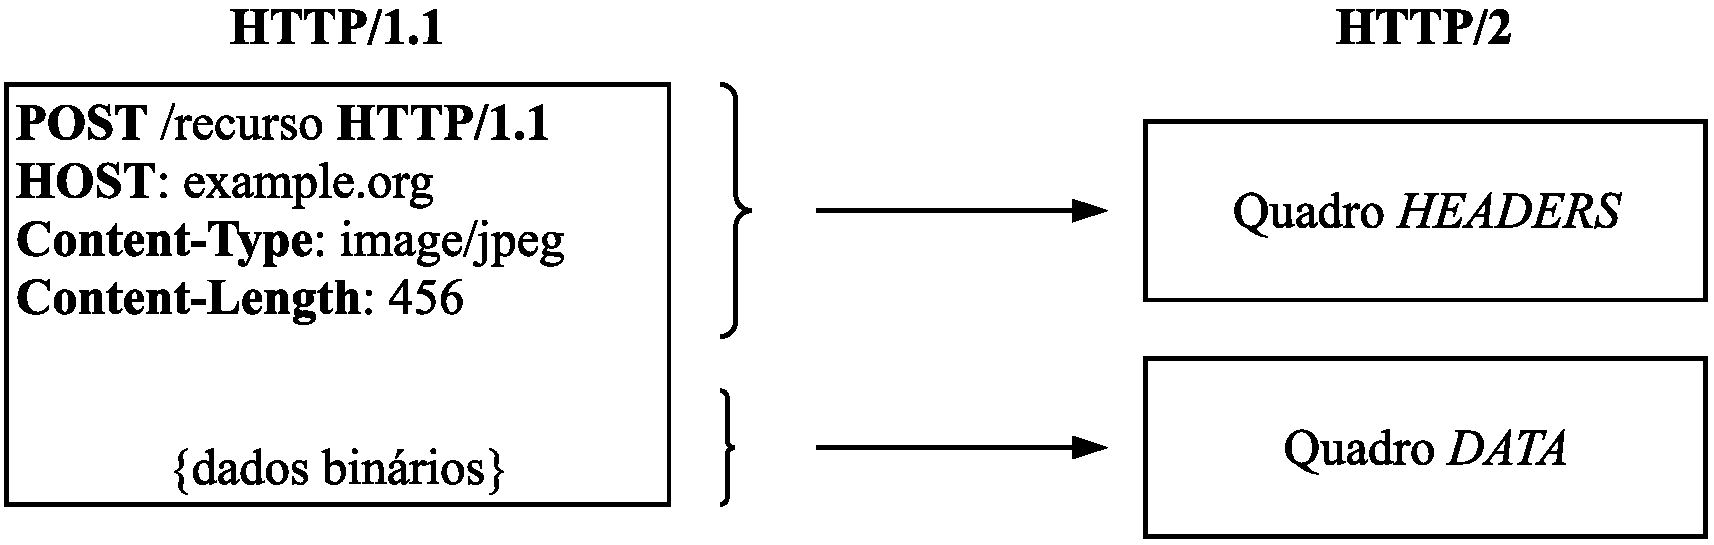
\includegraphics[width=\textwidth]{./fig/framing}
 \caption{Uma mensagem de requisição POST HTTP/1.1 e uma mensagem de requisição POST HTTP/2 equivalente.}
 \label{fig:framing}
\end{figure}

A especificação do HTTP/2 define um quadro como sendo a menor unidade de comunicação entre clientes e servidores. Um ou mais quadros podem ser enviados e recebidos tanto por clientes quanto servidores assim que o cliente inicia uma conexão TCP. Cada quadro é composto por um cabeçalho de tamanho fixo de 9 bytes seguido por um corpo de tamanho variado que depende do tipo do quadro.

\begin{figure}[hbt!]
 \centering
  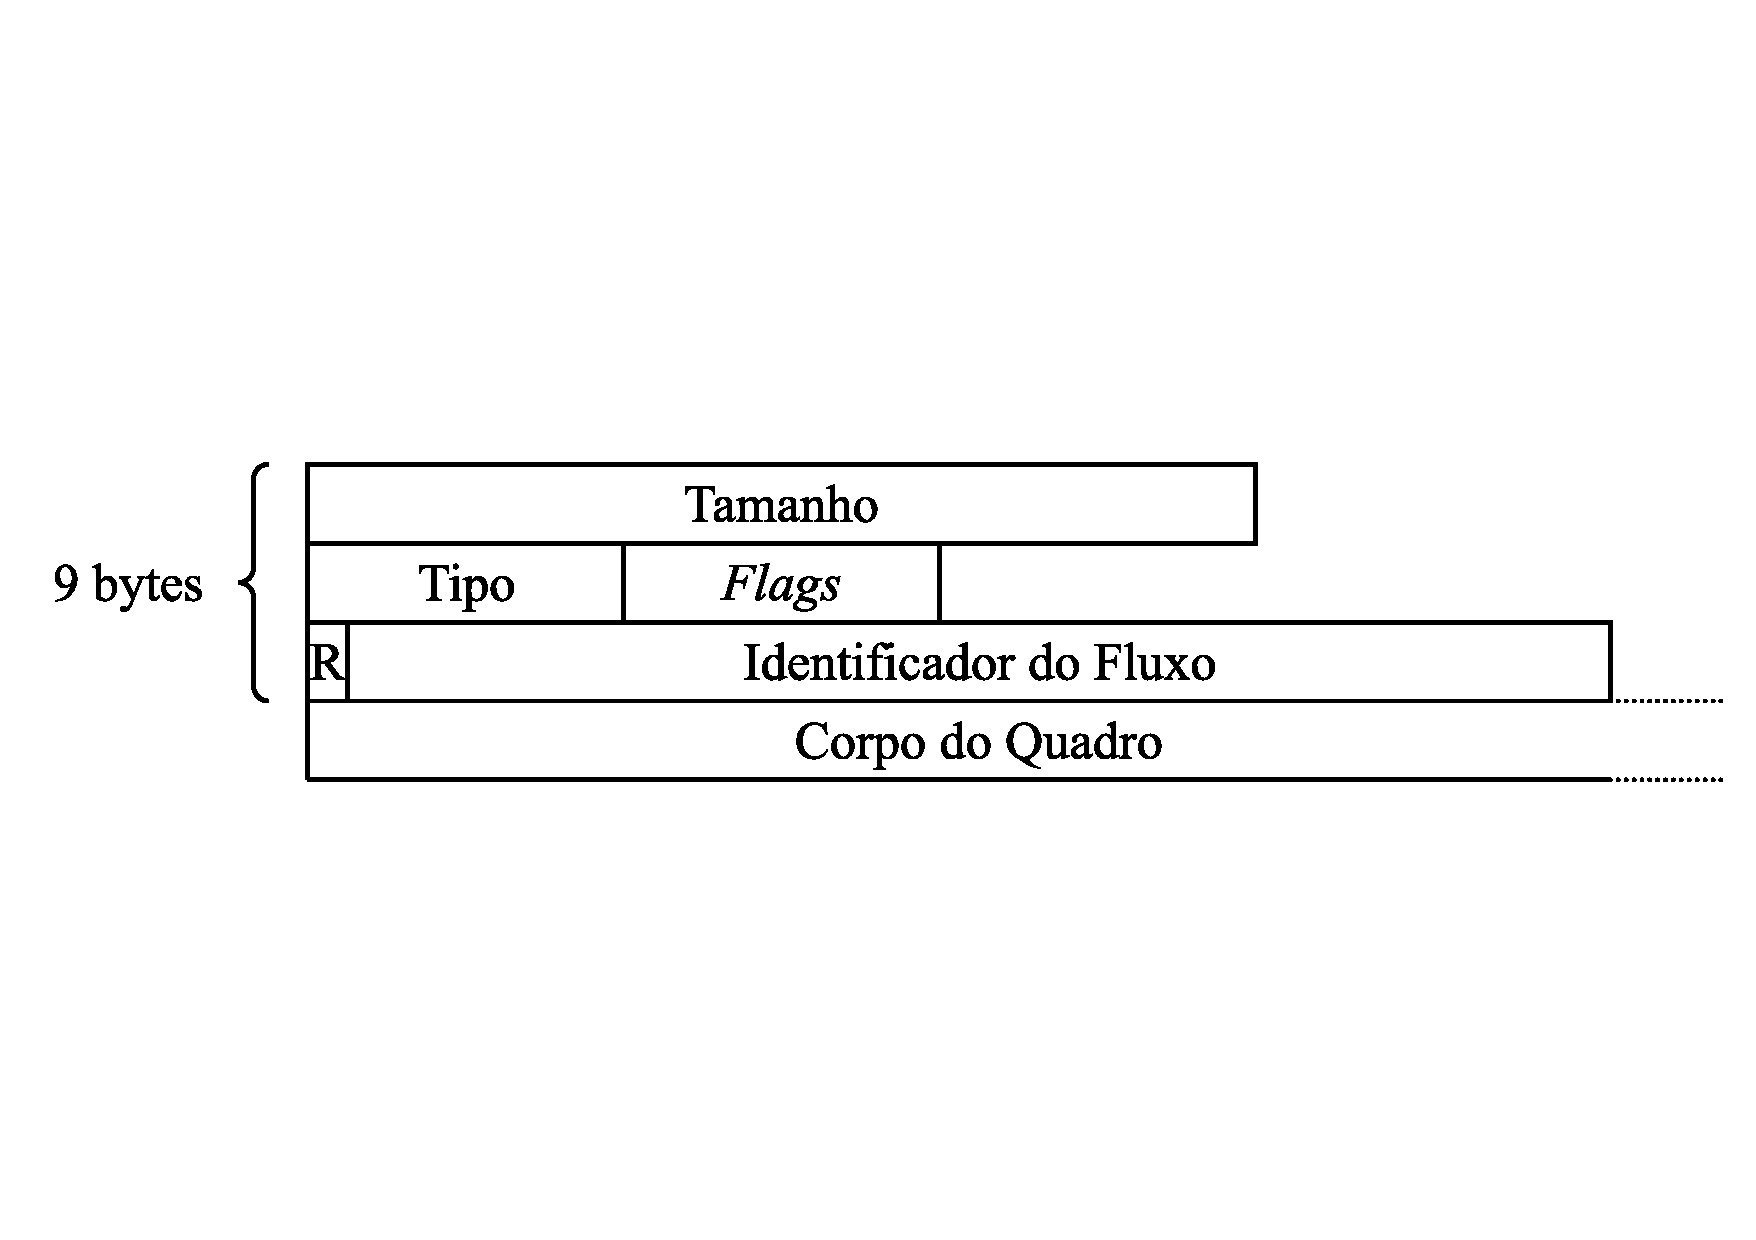
\includegraphics[width=\textwidth]{./fig/quadro}
 \caption{Formato de um quadro HTTP/2.}
 \label{fig:quadro}
\end{figure}

O formato de um quadro é mostrado na Figura \ref{fig:quadro}. O campo referente ao corpo do quadro varia em estrutura e conteúdo conforme o tipo do quadro. Os campos do cabeçalho do quadro são definidos como:

\begin{itemize}
    \item Tamanho (24 bits): carrega o tamanho do corpo do quadro (até $2^{24} - 1$ bytes).
    \item Tipo (8 bits): determina a estrutura e o conteúdo do corpo do quadro.
    \item {\em Flags} (8 bits): valor de 8 bits com significado específico para o tipo do quadro.
    \item R (1 bit): campo reservado que sempre possui valor 0.
    \item Identificador do Fluxo (31 bits): identifica unicamente um fluxo (ver Seção \ref{subsec:fluxos}).
\end{itemize}

Os seguintes tipos de quadros são definidos, cada um possuindo um papel distinto na comunicação HTTP/2:

\begin{itemize}
    \item {\em DATA}: transporta dados do corpo da mensagem.
    \item {\em HEADERS}: transporta campos de cabeçalhos da mensagem.
    \item {\em PRIORITY}: especifica a prioridade de um fluxo.
    \item {\em RST\_STREAM}: permite o fechamento de um fluxo.
    \item {\em SETTINGS}: transporta características de clientes e servidores para a conexão.
    \item {\em PUSH\_PROMISE}: sinaliza uma promessa para servir o recurso referenciado.
    \item {\em PING}: mede o RTT e verifica se uma conexão ociosa pode ser usada.
    \item {\em GOAWAY}: sinaliza o fechamento da conexão ou erros críticos.
    \item {\em WINDOW\_UPDATE}: permite implementação de controle de fluxo.
    \item {\em CONTINUATION}: continua uma sequência de campos de cabeçalhos.
\end{itemize}

\subsection{Fluxos de Mensagens}
\label{subsec:fluxos}

Um fluxo é definido como uma sequência independente e bidirecional de quadros dentro de uma conexão TCP e é identificado por um valor inteiro de 31 bits sem sinal. Tanto o cliente quanto o servidor podem criar e fechar um fluxo unilateralmente ou compartilhadamente entre si. Porém, clientes devem sempre criar um novo fluxo com valor {\em ímpar} maior que o valor do fluxo mais recentemente criado e servidores devem sempre criar um novo fluxo com valor {\em par} maior que o valor do fluxo mais recentemente criado. O fluxo de identificador 0 é reservado para controlar a conexão e não pode ser usado.

Clientes e servidores processam quadros de um fluxo na ordem em que são recebidos dentro da conexão TCP, podendo intercalar quadros de múltiplos fluxos concorrentemente abertos. Dessa forma, clientes e servidores são permitidos realizarem multiplexação de requisições e respostas associando cada troca de mensagens com um único fluxo.

Partindo do conhecimento da estrutura de um quadro, um fluxo pode ser examinado para que diferentes tipos de quadros sejam identificados, cada um com diferentes tamanhos. Como o tamanho é conhecido, o próximo quadro do fluxo pode ser processado mais eficientemente. Ao processar o cabeçalho do quadro, o seu corpo pode ser facilmente interpretado com base no seu tipo. Com isso, mensagens HTTP/2 são mais eficientes de serem processadas e mais compactas em transporte porque são binárias; mais robustas porque são menos propensas a erros; e mais simples porque existe apenas uma forma de processar uma mensagem.

\subsubsection{Ciclo de vida de um fluxo}

O ciclo de vida de um fluxo é exibido no diagrama da Figura \ref{fig:ciclo_fluxo}. As transições causam a mudança de um estado para outro de acordo com os quadros e {\em flags} enviados ou recebidos por clientes e servidores. Pressupõe-se que essas transições sejam geradas apenas pelo envio ou recebimento de quadros e {\em flags} ilustrados no diagrama. Por exemplo, não ocorre uma transição de estados quando quadros do tipo {\em CONTINUATION} seguem os quadros {\em HEADERS} ou {\em PUSH\_PROMISE} ou quando quadros do tipo {\em DATA} são enviados no estado aberto. Os estados são definidos como se segue:

\begin{itemize}
    \item ocioso: estado inicial de um fluxo.
    \item reservado (local): um cliente ou servidor {\em local} reservou um fluxo ocioso enviando um quadro do tipo {\em PUSH\_PROMISE}. 
    \item reservado (remoto): um cliente ou servidor {\em remoto} reservou um fluxo ocioso enviando um quadro do tipo {\em PUSH\_PROMISE}.
    \item aberto: estado onde clientes e servidores podem enviar quadros de qualquer tipo.
    \item semifechado (local): estado onde apenas quadros {\em WINDOW\_UPDATE}, {\em RST\_STREAM} e {\em PRIORITY} podem ser {\em enviados}, porém qualquer quadro pode ser {\em recebido}.
    \item semifechado (remoto): estado onde apenas quadros {\em WINDOW\_UPDATE}, {\em RST\_STREAM} e {\em PRIORITY} podem ser {\em recebidos}, porém qualquer quadro pode ser {\em enviado}. 
    \item fechado: indica o estado terminal de um fluxo, permitindo apenas o envio de quadros {\em PRIORITY}.
\end{itemize}

\begin{figure}[hbt!]
 \centering
  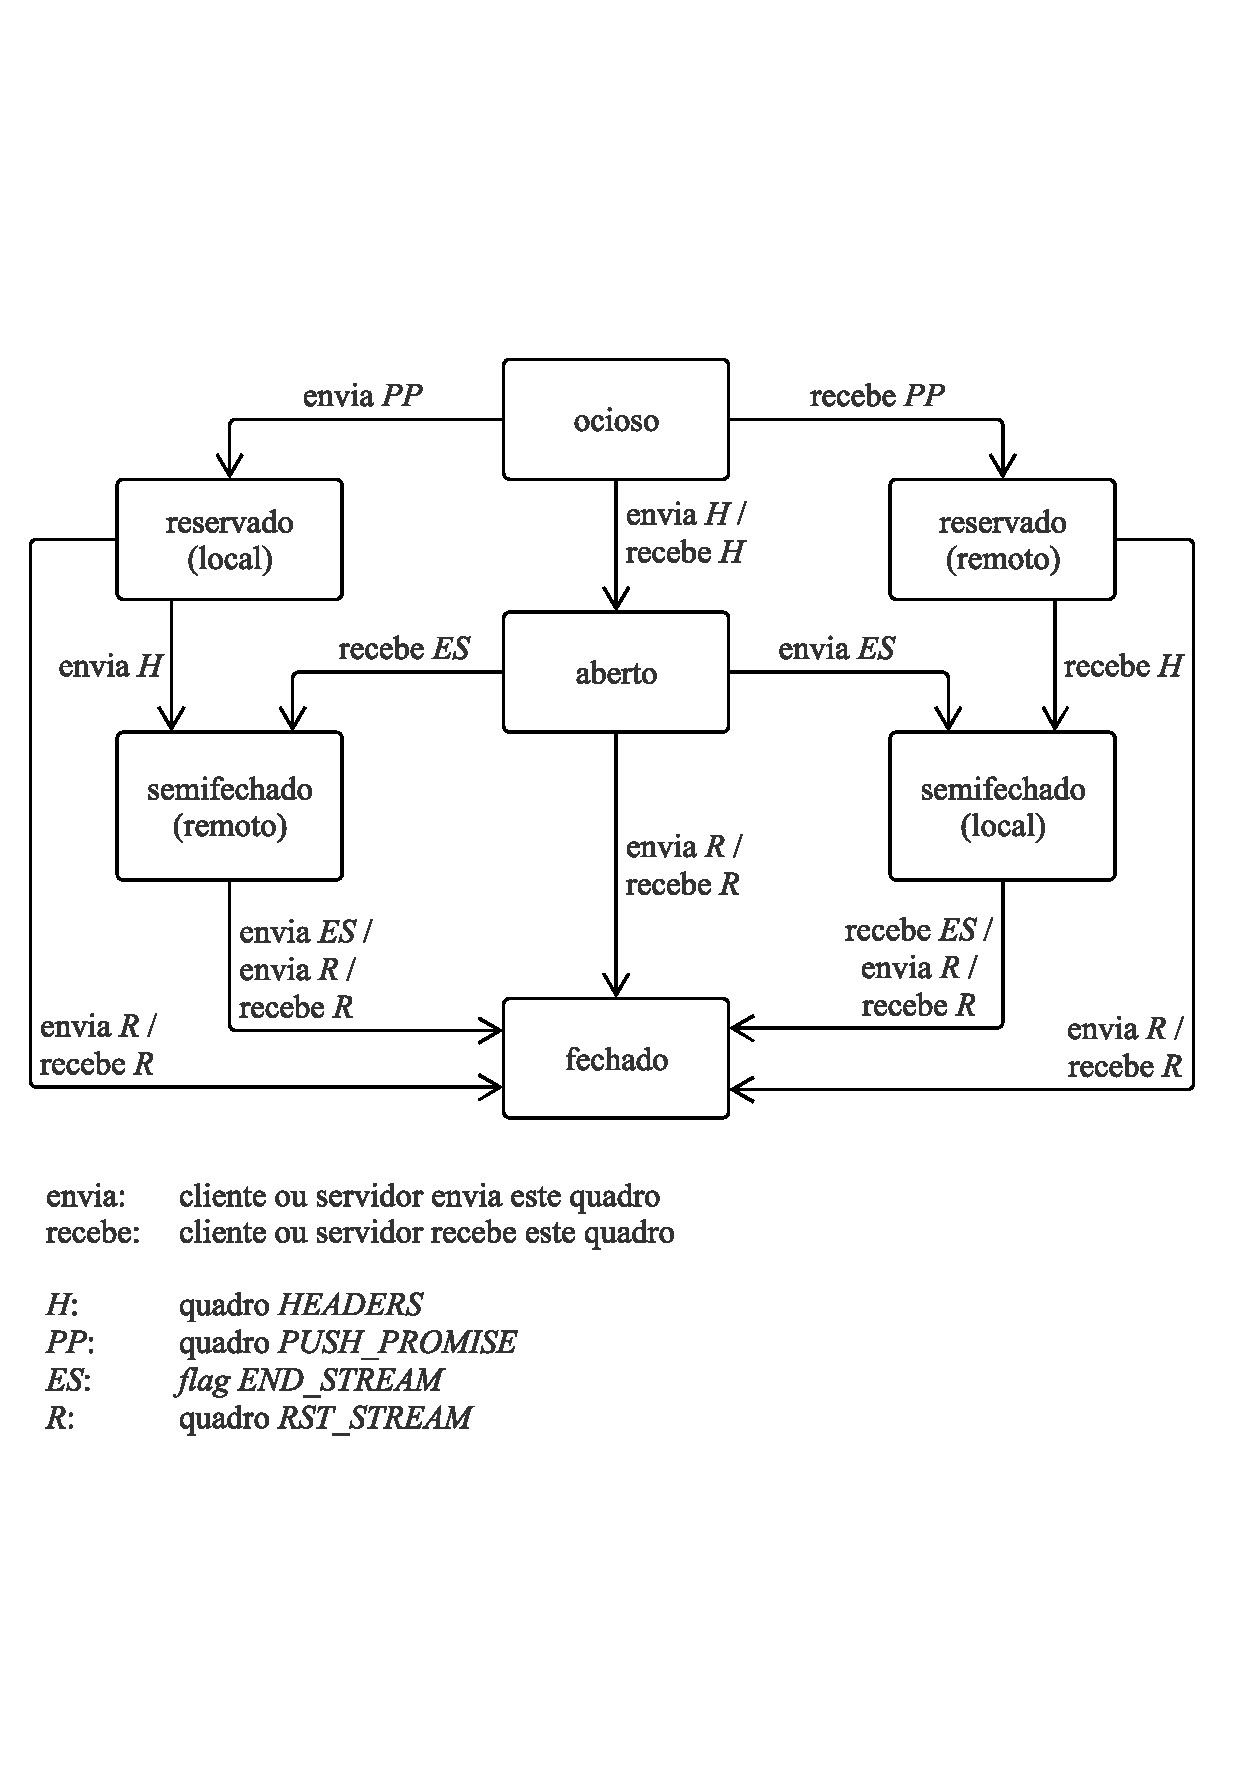
\includegraphics[width=\textwidth]{./fig/ciclo_fluxo}
 \caption{O ciclo de vida de um fluxo HTTP/2 ilustrado através de um diagrama com transição de estados.}
 \label{fig:ciclo_fluxo}
\end{figure}

\subsubsection{Controle de fluxo}

Se vários fluxos multiplexados (que carregam mensagens de requisição\slash resposta) estão sendo enviados pela conexão TCP, mas apenas um deles está entregando quadros, ele bloqueia outros fluxos. Visando resolver esse problema, um controle de fluxo é necessário para impedir que um fluxo interfira com outros fluxos, permitindo usá-los de modo mais eficiente. Para isso, a especificação do HTTP/2 define sete princípios de controle de fluxo, tais quais foram extraídos e traduzidos diretamente do documento RFC 7540 \cite{BelsheRFC7540}:

\begin{enumerate}
    \item O controle de fluxo é específico para uma conexão. Os dois tipos de controle de fluxo acontecem entre clientes e servidores em um único salto e não em todo o caminho de fim a fim.
    \item O controle de fluxo é implementado com o uso de quadros {\em WINDOW\_UPDATE} e é baseado em um esquema de créditos, já que cada destinatário (cliente ou servidor que está recebendo quadros) anuncia sua janela inicial (em bytes) que ele está preparado para receber em um fluxo e para toda a conexão. Essa janela é reduzida sempre que um remetente envia um quadro do tipo {\em DATA} e incrementado via quadros {\em WINDOW\_UPDATE} enviados pelo destinatário.
    \item O controle de fluxo é direcional com o controle geral fornecido pelo destinatário. Um destinatário pode optar por definir qualquer tamanho de janela que desejar para cada fluxo e para toda a conexão. Um remetente deve respeitar os limites de controle de fluxo impostos por um destinatário. Clientes, servidores e intermediários anunciam, independentemente, sua janela de controle de fluxo como um destinatário e cumprem os limites de controle de fluxo definidos por destinatários quando estiverem atuando como remetentes.
    \item O valor inicial da janela de controle de fluxo é de 65.535 bytes tanto para novos fluxos quanto para a conexão em geral.
    \item O tipo de quadro determina se o controle de fluxo se aplica a um quadro. Somente os quadros do tipo {\em DATA} estão sujeitos ao controle de fluxo; todos os outros tipos de quadro não consomem espaço na janela de controle de fluxo anunciada. Isso garante que estruturas de controle importantes não sejam bloqueadas pelo controle de fluxo.
    \item O controle de fluxo não pode ser desativado.
    \item O HTTP/2 define apenas o formato e a semântica do quadro {\em WINDOW\_UPDATE}. A especificação não estipula como um destinatário decide quando enviar esse quadro ou o valor que ele envia, nem como um remetente escolhe enviar pacotes. As implementações são capazes de selecionar qualquer algoritmo que atenda às suas necessidades.
\end{enumerate}

Ainda de acordo com a especificação, as implementações também são responsáveis por gerenciar como as requisições e as respostas são enviadas com base na prioridade, escolhendo como evitar o bloqueio de requisições e gerenciar a criação de novos fluxos. As escolhas de algoritmo para estas poderiam interagir com qualquer algoritmo de controle de fluxo. Os remetentes sempre estão sujeitos a respeitar a janela de controle de fluxo anunciada pelo destinatário, mas destinatários que não desejarem controle de fluxo podem anunciar uma janela de tamanho máximo ($2^{31} - 1$) e podem manter essa janela enviando um quadro {\em WINDOW\_UPDATE} quando qualquer quadro {\em DATA} é recebido.

\subsection{HPACK: Compressão de Cabeçalhos}
\label{subsec:compression}

Para toda requisição\slash resposta do HTTP/1.1, os mesmos cabeçalhos extensos e redundantes são enviados e recebidos durante uma conexão TCP. Isso resulta em problemas de congestionamento de rede. Para resolver isso, um padrão de compressão de cabeçalhos HTTP/2 para um formato binário foi aprovado pela IETF, denominado HPACK \cite{BelsheRFC7541}.

A especificação do HTTP/2 define listas de cabeçalhos como zero ou mais campos de cabeçalhos. Campos de cabeçalhos são os tradicionais nomes com um ou mais valores associados. Essas listas são serializadas em um bloco de cabeçalhos utilizando os algoritmos definidos em HPACK. Esse bloco de cabeçalhos é então dividido em uma ou mais cadeias de bytes e carregadas no corpo de quadros {\em HEADERS}, {\em PUSH\_PROMISE} ou {\em CONTINUATION}. Um cliente ou um servidor que está recebendo esses cadeias de bytes os concatenam e depois descomprimem o bloco para reconstruir a lista decodificada.  Os principais elementos do HPACK são os seguintes \cite{Yamamoto:2017:EHH:3095786.3095787}:

\begin{itemize}
    \item Campo de cabeçalhos.
    \item Bloco de cabeçalhos.
    \item Tabela estática.
    \item Tabela dinâmica.
    \item Codificador.
    \item Decodificador.
\end{itemize}

Um campo de cabeçalho é um par (nome, valor), que são uma sequência de bytes. Campos de cabeçalhos codificados são representados ou como um valor numérico (índice) ou como um valor literal. Na representação de índice, existe uma referência para uma entrada na tabela estática ou na tabela dinâmica. Na representação literal, existe um par (nome, valor) onde um nome ou é representado literalmente ou é uma referência para uma entrada na tabela estática ou na tabela dinâmica e um valor é representado literalmente.

Um bloco de cabeçalho é uma concatenação de representações de campos de cabeçalhos descritos no parágrafo anterior. Um decodificador pode processar um bloco de cabeçalho sequencialmente para reconstruir a lista de cabeçalhos original.

Uma tabela estática é uma estrutura de dados do tipo lista e é predefinida em \cite{BelsheRFC7541} com uma lista estática de campos de cabeçalhos, podendo ser referenciada por um índice cujos valores são pares (nome do cabeçalho, valor do cabeçalho). Por exemplo, o índice 2 possui o par (``:method'', ``GET'') e o índice 19 possui o par (``accept'', `'), sem valor do cabeçalho. A tabela estática associa estaticamente campos de cabeçalhos que ocorrem frequentemente para índices. Trata-se de uma tabela ordenada, de apenas leitura ({\em read-only}), é sempre acessível e compartilhada em todos os contextos de codificação e decodificação.

Uma tabela dinâmica é uma estrutura de dados similar à tabela estática, com a diferença de que as entradas são criadas dinamicamente. Ela tem um limite superior ao seu tamanho e se a criaçao de novas entradas ultrapassar esse tamanho, as entradas mais antigas são removidas. Clientes e servidores mantêm uma tabela dinâmica para o envio e outra para o recebimento de campos de cabeçalhos (correspondem a contextos de codificação e decodificação, respectivamente). Elas operam seguindo o princípio FIFO ({\em First In, First Out}) e associam campos de cabeçalhos para índices e é específica para um contexto de codificação\slash decodificação. As tabelas dinâmicas podem ser usadas pelo codificador para indexar campos de cabeçalhos redundantes e é permitido que ela contenha entradas duplicadas.

O codificador é implementado com o auxílio das tabelas estáticas e dinâmicas que mapeiam campos de cabeçalhos para índices. Sua função é atualizar a tabela dinâmica e ordenar os campos de cabeçalho no bloco de cabeçalho de acordo com a ordem original da lista de cabeçalho. Na verdade, existem três métodos de compressão utilizados pelo codificador para codificar campos de cabeçalhos: tabelas estáticas, tabelas dinâmicas e código de Huffman estático. Já o decodificador compartilha as modificações prescritas pelo codificador e mantém uma tabela dinâmica como um contexto de decodificação para descomprimir blocos de cabeçalhos.

\subsection{Priorização de Requisições}
\label{subsec:priority}

Priorizar uma requisição é permitir que clientes informem a quantidade de recursos (como CPU, memória e taxas de transmissão de dados) que devem ser alocados a essa requisição em relação a outras requisições. Visto que vários fluxos carregando requisições podem estar concorrentemente abertos em uma comunicação HTTP/2, clientes podem atribuir informações de priorização para um fluxo específico quando ele é aberto (enviando um quadro do tipo {\em HEADERS}) e em qualquer momento da comunicação essa prioridade pode ser alterada enviando um quadro do tipo {\em PRIORITY}.

Para isso, o HTTP/2 permite que dependências por um fluxo sejam associados a um outro fluxo que depende do seu término. Caso dois ou mais fluxos sejam dependentes do término do mesmo fluxo, um peso (um número inteiro entre 1 e 256) pode ser atribuído para cada fluxo dependente para informar que os recursos disponíveis devem ser alocados em proporção aos seus pesos.

O mecanismo de dependências e pesos de fluxos para permitir priorização pode ser ilustrado através de uma árvore de dependências. Por exemplo, considere a árvore de dependências da Figura \ref{fig:dependency_tree}. Cada nó representa um fluxo, sendo que o número fora dos parênteses é o seu identificador e o número dentro dos parênteses é o seu peso.

\begin{figure}[hbt!]
 \centering
  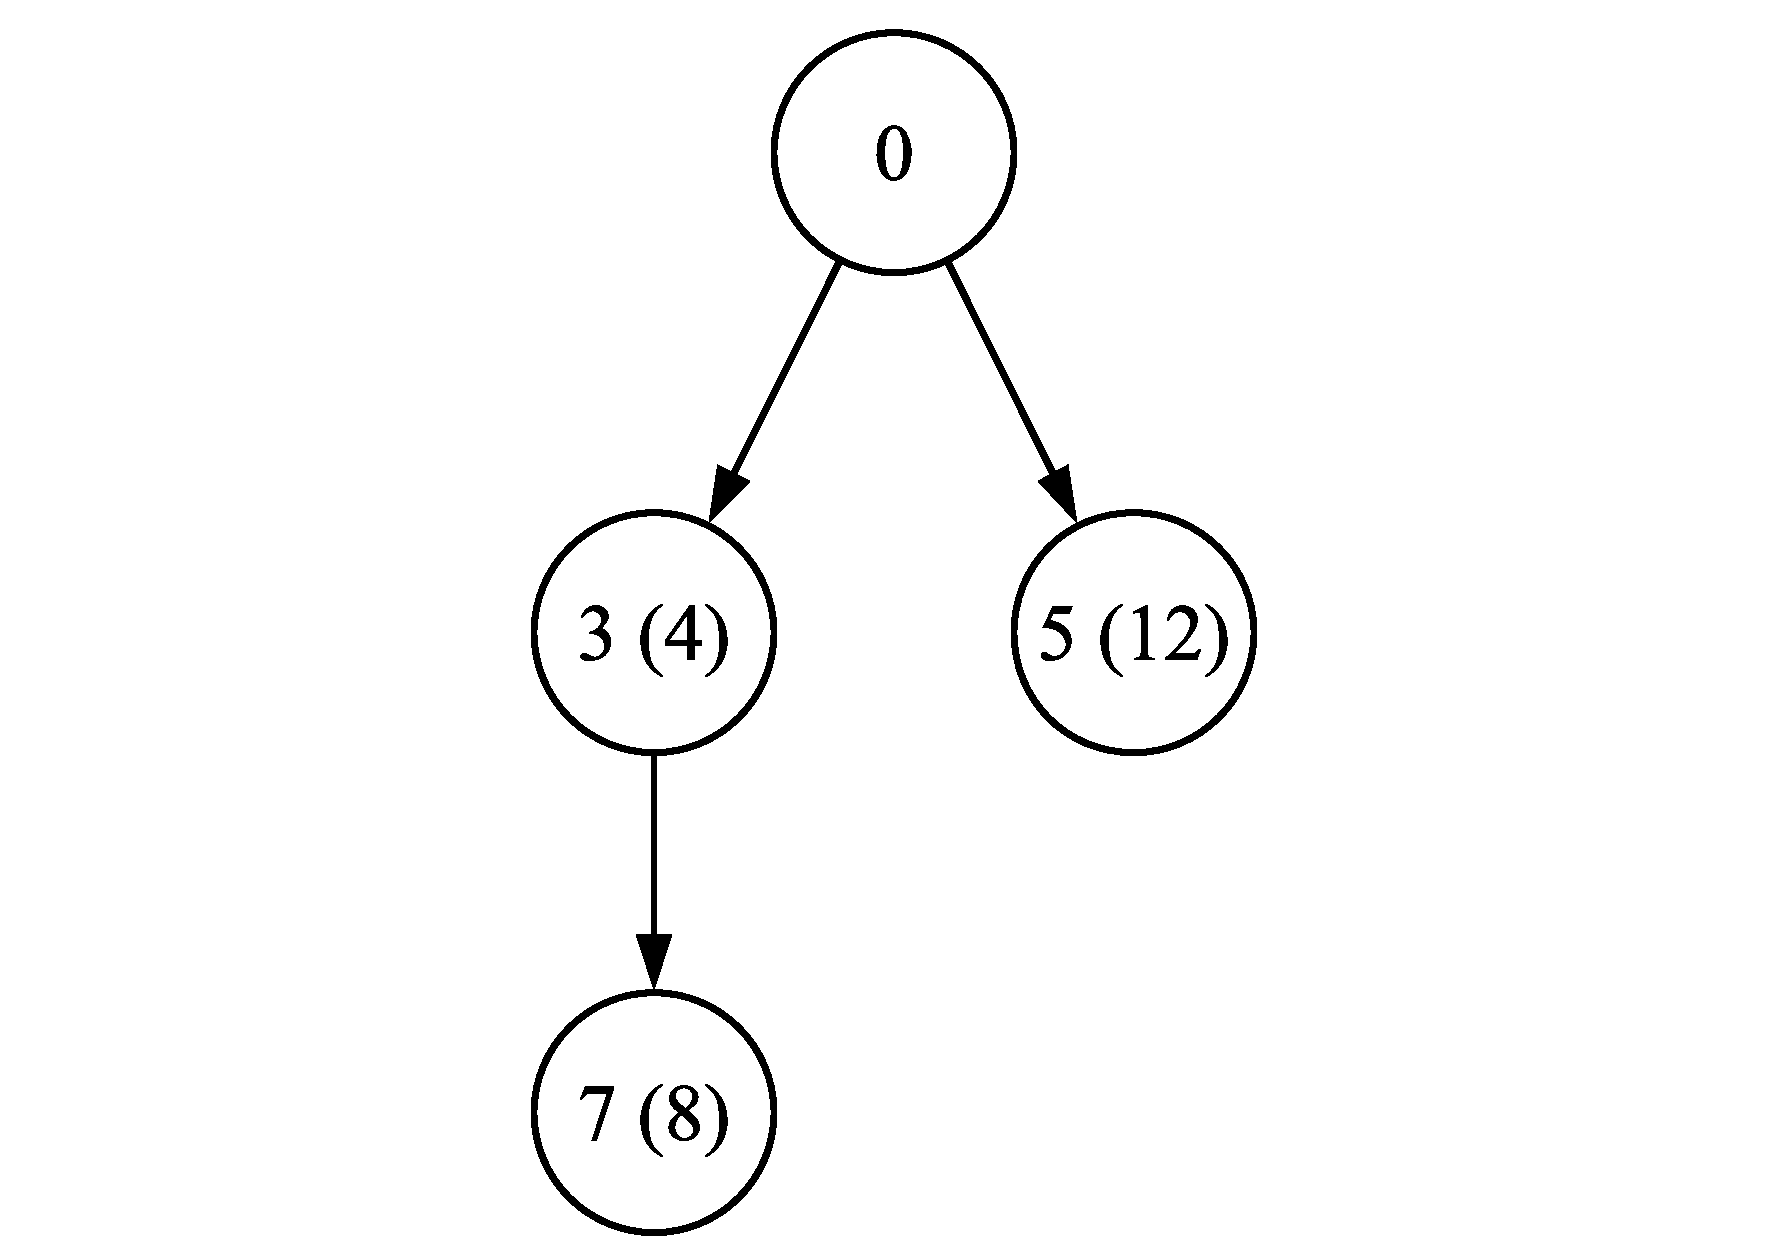
\includegraphics[width=0.5\textwidth]{./fig/dependency_tree}
 \caption{Dependências e pesos de fluxos HTTP/2 como uma árvore de dependências.}
 \label{fig:dependency_tree}
\end{figure}

Todo fluxo que não tem dependência declarada depende do fluxo 0 (conforme visto na subseção \ref{subsec:fluxos}, um fluxo de valor 0 é reservado para a conexão), que forma a raiz da árvore. Sendo assim, os fluxos 3 e 5 dependem do fluxo 0 e o fluxo 7 depende do fluxo 3. Como os fluxos 3 e 5 são dependentes do mesmo fluxo, a alocação de recursos é distribuída proporcionalmente em relação aos seus pesos: o fluxo 3 recebe 1/4 (4/16) e o fluxo 5 recebe 3/4 (12/16) dos recursos disponíveis.

\subsection{{\em Push} de Requisição\slash Resposta do Servidor}
\label{subsec:push}

Uma página Web típica inclui vários recursos independentes e que precisam ser requisitados separadamente por um cliente HTTP. Por exemplo, o arquivo HTML padrão de um servidor (comumente referido como {\em index.html}) pode incluir recursos dinâmicos como arquivos JavaScript, CSS e imagens que são necessários para exibir a página corretamente. No HTTP, o cliente precisa requisitar cada um desses recursos separadamente.

No HTTP/2, um servidor pode enviar várias respostas para uma única requisição de um cliente, ou seja, um servidor pode fazer um {\em push} (forçar) o envio de duas ou mais respostas contendo recursos associados a requisição original por um recurso, sem que clientes tenham que requisitar cada recurso separadamente. Assim, o servidor pode enviar antecipadamente todos os recursos dinâmicos contidos em uma página, sem que o cliente precise requisitar cada um.

O {\em push} do servidor é dividido em {\em push} de requisição e {\em push} de resposta. No {\em push} de requisição, o servidor envia um quadro do tipo {\em PUSH\_PROMISE} junto com campos de cabeçalhos (assim como nos cabeçalhos de uma requisição normal de um cliente) no estado ocioso de um fluxo, indicando que esse fluxo será reservado para um futuro {\em push} de resposta. Depois de enviado esse quadro, o servidor começa a enviar respostas assim que uma requisição tenha sido explicitamente feita pelo cliente.

É importante observar que o cliente pode desabilitar o {\em push} do servidor e que, por medidas de segurança, o servidor precisa ser autoritativo pelas respostas enviadas. O cliente também pode optar por recusar um {\em push} do servidor enviando um quadro do tipo {\em RST\_STREAM}. Assim, o cliente tem completo controle sobre como o {\em push} do servidor é usado.

\section{Lua}
\label{sec:lua}

A linguagem de programação Lua \cite{Ierusalimschy:2009:PMP:2175094.2175096, Ierusalimschy2016PiL, Ierusalimschy2018:LDL:3289258.3186277}  foi criada no início dos anos 1990 por Roberto Ierusalimschy, Waldemar Celes e Luis Henrique de Figueiredo na Pontifícia Universidade Católica do Rio de Janeiro (PUC-Rio). É uma linguagem de {\em scripting} multiparadigma que oferece suporte principalmente ao paradigma de programação procedural, embora também seja usada em programação concorrente, programação orientada a objetos, programação funcional, entre outros paradigmas. Lua também oferece suporte à descrição de dados, no estilo de JSON ou XML.

Atualmente, Lua é utilizada em várias aplicações industriais, com uma ênfase em sistemas embarcados e jogos, sendo a linguagem de {\em scripting} mais utilizada em jogos do mundo. Ela também é considerada uma das linguagens de {\em scripting} de melhor desempenho do mundo, devido a sua implementação eficiente.

Lua tem tipagem dinâmica, estruturas de dados dinâmicas, gerenciamento automático de memória e outras construções de linguagem similares às de outras linguagens de {\em scripting} dinamicamente tipadas. O que separa Lua unicamente dessas linguagens é o seu projeto, que foi definido em função dos seguintes objetivos:

\begin{itemize}
    \item Extensibilidade: Lua é uma biblioteca escrita em C e possui uma API C usada tanto para ser estendida com novas características quanto para estender outras aplicações escritas em C. De fato, a extensibilidade impactou fortemente o projeto de Lua \cite{Ierusalimschy2011passing}.
    \item Simplicidade: Lua é uma linguagem simples e pequena. Ao invés de ter incontáveis construções de linguagem feitas para resolver um determinado problema, Lua possui poucos (mas flexíveis) conceitos que atendem diferences necessidades.
    \item Eficiência: A implementação de Lua é pequena em tamanho. Isso a torna uma implementação muito eficiente e portátil. Como Lua é leve e eficiente, uma aplicação que embute Lua não é sobrecarregada.
    \item Portabilidade: Lua pode ser executada em praticamente todas as plataformas existentes por ser escrita em ANSI (ISO) C. Por ser pequena, Lua executa facilmente nessas plataformas sem que elas sejam negativamente impactadas.
\end{itemize}

\subsection{Tabelas e Funções}
\label{subsec:tables}

Lua é bastante reconhecida por sua simplicidade em harmonia com sua flexibilidade de programação. Muitas construções da linguagem são criadas a partir de duas construções mais básicas: tabelas e funções. Ambas construções permeiam toda a linguagem e formam a base para mecanismos mais complexos como módulos e programação orientada a objetos.

A tabela é uma estrutura de dados dinâmica e constitui a única estrutura de dados de Lua. As tabelas de Lua são semelhantes aos vetores associativos de Perl e PHP, que são compostas por pares (chave, valor). É fácil pensar em uma tabela como um {\em map} ou como uma tabela {\em hash} por associarem uma chave a um valor. Tabelas são usadas para implementar as mais diversas estruturas de dados (tais como vetores, registros, listas, filas, pilhas e conjuntos) de modo eficiente e são as construções que permitem criar outras construções mais complexas da linguagem. Logo, tabelas permeiam toda a linguagem Lua.

Lua suporta diferentes mecanismos para construir tabelas. A expressão \verb|t["x"] = 1| cria uma tabela \verb|t| onde a chave \verb|"x"| é associada ao valor 1 e a expressão \verb|t[1] = "x"| cria uma tabela \verb|t| associando a chave 1 ao valor \verb|"x"|. Utilizando o chamado ``açúcar sintático'' de Lua, a primeira expressão pode ser escrita como \verb|t.x = 1|. Utilizando a sintaxe de construtor \verb|{}|, o construtor \verb|{x = 1, y = 2}| cria uma tabela com duas entradas, uma associando \verb|"x"| ao valor 1 e outra associando \verb|"y"| ao valor 2 \cite{Ierusalimschy2018:LDL:3289258.3186277}.

As funções de Lua têm funcionalidades tradicionais às de outras linguagens de programação, mas com o diferencial de que elas são valores de primeira classe, isto é, uma função pode ser armazenada em variáveis, passada como argumento para parâmetros de outras funções e ser retornada como resultado dessas outras funções. Lua também oferece suporte a funções com escopo léxico ({\em closures}), habilitando Lua a ser utilizada para programação funcional. O código abaixo mostra uma função anônima sendo atribuída a variável \verb|mod|:

\begin{Verbatim}
mod = function(x, y)
  return x % y
end
\end{Verbatim}

Tabelas e funções de primeira classe podem ser usados para implementar módulos em Lua (semelhantes a pacotes em Java e Perl, ou {\em namespaces} em C++), que servem como bibliotecas ou como um espaço de nomes para a linguagem. Por exemplo, considere o Código \ref{code:ponto}, que mostra como uma biblioteca simples em Lua que permite criar pontos (coordenadas) e calcular a distância entre dois pontos pode ser criada. Um programador pode (re)usar essa biblioteca usando a função \verb|require| da biblioteca padrão (Código \ref{code:test_ponto}).

\begin{center}
 \begin{minipage}{0.7\textwidth}
  \begin{codigo}[H]
   \small
   \VerbatimInput[xleftmargin=10mm,numbers=left,obeytabs=true]{./prog/ponto.lua}
   \caption{\texttt{Biblioteca "ponto"}}
   \label{code:ponto}
  \end{codigo}
 \end{minipage}
\end{center}

\begin{center}
 \begin{minipage}{0.7\textwidth}
  \begin{codigo}[H]
   \small
   \VerbatimInput[xleftmargin=10mm,numbers=left,obeytabs=true]{./prog/test_ponto.lua}
   \caption{\texttt{Utilizando a biblioteca "ponto"}}
   \label{code:test_ponto}
  \end{codigo}
 \end{minipage}
\end{center}

A função \verb|require| mostrada na linha 1 do Código \ref{code:test_ponto} é um exemplo de uma das funções fornecidas pela biblioteca padrão de Lua. Além dessa função, a função \verb|math.sqrt| é exibida na linha 10 do Código \ref{code:ponto}, que faz parte da biblioteca padrão \verb|math| de Lua. A biblioteca ``ponto'' é um exemplo de uma biblioteca externa que pode ser criada por programadores Lua como forma de estender as funcionalidades da linguagem. Elas não vêm inclusas no conjunto de bibliotecas padrões de Lua e devem ser incluídas manualmente no código caso o programador deseje usá-la.

Tabelas e funções também podem ser utilizadas para simular programação orientada a objetos. Conceitos de orientação a objetos como classes, objetos, métodos e herança podem ser representados por tabelas e funções, seguindo o padrão de utilizar mecanismos básicos da linguagem para construir mecanismos mais complexos.

Por exemplo, considere o Código \ref{code:class}, onde uma classe nomeada {\em class} é implementada em Lua. Essa classe faz o uso de dois métodos: \verb|set_value(value)| define um novo valor \verb|value| e \verb|get_value()| recupera esse valor. Um construtor \verb|new| também é definido para instanciar objetos dessa classe. Lua possibilita a criação de classes com o auxílio da função \verb|setmetatable| para instanciar tabelas a partir de outras tabelas e do metamétodo \verb|__index| para acessar valores dessas tabelas. Além disso, Lua provê o ``açúcar sintático'' de dois-pontos para criar um parâmetro de autoreferência (normalmente chamado de {\em this} ou {\em self} em outras linguagens de programação orientadas a objetos).

O Código \ref{code:object} mostra como um objeto pode ser instanciado a partir de uma classe (representada por um módulo). Na linha 3, o código cria um novo objeto a partir da classe \verb|class| utilizando seu construtor \verb|new|, configura o valor 2 para esse objeto e depois recupera esse mesmo valor chamando os métodos da classe \verb|class|.

\begin{center}
 \begin{minipage}{0.7\textwidth}
  \begin{codigo}[H]
   \small
   \VerbatimInput[xleftmargin=10mm,numbers=left,obeytabs=true]{./prog/class.lua}
   \caption{\texttt{Classe}}
   \label{code:class}
  \end{codigo}
 \end{minipage}
\end{center}

\begin{center}
 \begin{minipage}{0.7\textwidth}
  \begin{codigo}[H]
   \small
   \VerbatimInput[xleftmargin=10mm,numbers=left,obeytabs=true]{./prog/object.lua}
   \caption{\texttt{Objeto}}
   \label{code:object}
  \end{codigo}
 \end{minipage}
\end{center}

\subsection{Co-rotinas}
\label{subsec:coroutines}

O suporte à programação concorrente em Lua é fornecido por co-rotinas e funcionam como {\em multithreading} cooperativa: apenas uma co-rotina ({\em thread}) está em execução por vez, e a troca de contexto entre as co-rotinas é feita de forma explícita. Diferentemente de {\em multithreading} preemptiva, onde a troca de contexto entre as {\em threads} ocorre de forma implícita, na cooperativa existem funções explícitas para a transferência de controle.

Co-rotinas são, assim como funções, valores de primeira classe. Outra característica de co-rotinas em Lua é que elas são assimétricas, ou seja, existe uma função para suspender uma co-rotina e outra função para executar uma co-rotina. Isso as distingue de co-rotinas simétricas, onde apenas uma função exerce esse papel.

Uma co-rotina é criada através da biblioteca padrão \verb|coroutine| de Lua. Assim como a biblioteca padrão \verb|table| de Lua, a biblioteca \verb|coroutine| é um módulo nativo da linguagem Lua, consistindo de tabelas e funções. As principais funções que fazem parte do módulo \verb|coroutine| são:

\begin{itemize}
    \item \verb|coroutine.create|: cria uma co-rotina.
    \item \verb|coroutine.yield|: suspende uma co-rotina.
    \item \verb|coroutine.resume|: coloca uma co-rotina em execução.
    \item \verb|coroutine.status|: verifica o estado de uma co-rotina.
\end{itemize}

O funcionamento de uma co-rotina pode ser ilustrado através de um exemplo de código. No Código \ref{code:coroutine}, que foi adaptado de \cite{Ierusalimschy2018:LDL:3289258.3186277}, uma co-rotina é criada na linha 1 pela função \verb|coroutine.create|, passando uma função anônima como seu parâmetro. Essa função apenas cria a co-rotina, sem executá-la. Na linha 2, o valor de \verb|x| passado como parâmetro será 1 porque a função \verb|coroutine.resume| na linha 8 passou esse valor como argumento. Na linha 3, a co-rotina suspende a execução, passando o valor 2 como argumento de \verb|coroutine.yield| para \verb|coroutine.resume| na linha 8 e armazenando esse valor na variável \verb|y|. Depois, o programa retorna a executar a co-rotina, dessa vez passando o valor 3 como argumento de \verb|coroutine.resume| na linha 9 para o retorno de \verb|coroutine.yield| na linha 3. Por fim, a co-rotina causa o término de \verb|coroutine.resume| na linha 9 retornando o valor 4 e armazenando-o na variável \verb|y|.

\begin{center}
 \begin{minipage}{0.7\textwidth}
  \begin{codigo}[H]
   \small
   \VerbatimInput[xleftmargin=10mm,numbers=left,obeytabs=true]{./prog/coroutine.lua}
   \caption{\texttt{Co-rotina}}
   \label{code:coroutine}
  \end{codigo}
 \end{minipage}
\end{center}

Uma desvantagem em utilizar co-rotinas é que gerenciá-las pode se tornar uma tarefa complexa quando o número de suspensões e retomadas aumentam. Por exemplo, se uma co-rotina invoca uma operação bloqueantes de rede como \verb|receive| e bloqueia, todo o programa é bloqueado até que a operação termine. Esse comportamento pode ser evitado fornecendo um conjunto de funções não bloqueantes que iniciam uma operação de rede e suspende a co-rotina ativa quando a operação não puder ser imediatamente completada.

Ierusalismchy \cite{Ierusalimschy2016PiL} mostra um exemplo de uma aplicação concorrente que utiliza co-rotinas com funções não bloqueantes da API {\em socket} do LuaSocket \cite{Nehab2007}. Uma outra forma de evitar esse comportamento indesejável em aplicações concorrentes é criando um escalonador de co-rotinas, que gerencia a tarefa de suspender e executar co-rotinas quando as operações de rede bloquearem. Uma biblioteca em Lua que proporciona essa funcionalidade é chamada Copas, descrita na seção a seguir.

\subsection{Copas}
\label{subsec:copas}

Copas ({\em Coroutine Oriented Portable Asynchronous Services for Lua}) \cite{Copas} é uma biblioteca que oferece suporte a operações assíncronas para aplicações de rede escritas em Lua e seu foco é na criação de clientes e servidores. Funções assíncronas são fornecidas pela biblioteca Copas para impedir que a aplicação de rede fique bloqueada em uma chamada de rede tipicamente bloqueante (por exemplo, na função de recebimento de dados \verb|receive|). Para isso, Copas faz uso da característica de {\em multithreading} cooperativa de Lua, atuando como um escalonador de co-rotinas.

Copas utiliza a biblioteca LuaSocket \cite{Nehab2007} para interagir com sua API {\em socket}. Com funcionamento semelhante às funções \verb|socket.send| e \verb|socket.receive| do LuaSocket, a função \verb|copas.send| envia dados pelo {\em socket} e a função \verb|copas.receive| recebe dados pelo {\em socket}. A diferença entre essas funções em ambas as bibliotecas é que em Copas não existem chamadas bloqueantes. O uso de {\em multithreading} cooperativa de Lua permite que os envios e recebimentos de dados pelo {\em socket} sejam tratados de forma simultânea em várias {\em threads}, desde que elas façam chamadas às funções \verb|copas.send| e \verb|copas.receive| de Copas.

A tarefa de escalonar co-rotinas é realizada pelo escalonador do Copas, onde um {\em loop} principal fica responsável principalmente por empregar um mecanismo de consulta para verificar se o resultado da computação de uma função não bloqueante de um {\em socket} (por exemplo, recebimento de dados ou {\em time out}) já está disponível. Quando o resultado é recebido, o escalonador utiliza co-rotinas para processá-lo concorrentemente com outras co-rotinas contendo resultados de computação de outras funções não bloqueantes. Com isso, a execução assíncrona de uma aplicação de rede é alcançada, pois o uso de funções não bloqueantes de um {\em socket} em combinação com a facilidade de executá-las concorrentemente com várias {\em threads} nunca travam o {\em loop} principal da aplicação. As seguintes funções de Copas implementam esse gerenciamento de co-rotinas:

\begin{itemize}
    \item \verb|copas.loop|: inicia o {\em loop} principal do Copas.
    \item \verb|copas.addthread|: adiciona uma nova co-rotina ao escalonador para que ele possa escalonar essa co-rotina quando o resultado de uma computação assíncrona de rede for recebida.
    \item \verb|copas.sleep|: assim como a função \verb|coroutine.yield| vista na Subseção \ref{subsec:coroutines}, suspende a execução da co-rotina atual (apenas uma pode estar em execução) criada por \verb|copas.addthread|.
    \item \verb|copas.wakeup|: volta a executar a co-rotina criada por \verb|copas.addthread| e passada como parâmetro para essa função.
\end{itemize}

Para ilustrar um caso de uso do Copas, considere o Código \ref{code:repetidor}, que demonstra um simples uso de um repetidor que transmite de volta os dados recebidos e termina quando recebe \verb|quit|. Para simplificar, o código para criação do {\em socket} que utiliza a API do LuaSocket foi omitido. Primeiramente, nas linhas 19 e 20, as {\em threads} \verb|on_quit| e \verb|despachante| são adicionadas ao escalonador do Copas, respectivamente. A {\em thread} \verb|despachante| é simplesmente um {\em loop} que recebe dados provenientes de um {\em socket} e verifica se esses dados correspondem a \verb|quit|, sinalizando o término do envio de dados. A {\em thread} \verb|on_quit| é uma tratadora dessa sinalização de \verb|quit|, que é despachada quando os dados param de ser enviados.

Depois de adicionadas as {\em threads}, o {\em loop} principal do Copas começa a executar, na linha 22. A primeira {\em thread} que ele escalona é \verb|on_quit|, pois foi a primeira a ser adicionada. Em seguida, na linha 14, essa {\em thread} é colocada em modo suspenso porque ela só poderá ser despachada quando os dados pararem de serem enviados pelo {\em socket}, ou seja, quando \verb|quit| é recebido. Assim que a {\em thread} \verb|on_quit| é suspendida, a {\em thread} \verb|despachante| é escalonada pelo {\em loop} principal, que começa a verificar pela sinalização do término do envio de dados. Caso os dados ainda estejam sendo enviados pelo remetente, esses mesmos dados são enviados para o mesmo, repetindo o ciclo. Quando os dados correspondentes a \verb|quit| são recebidos, a {\em thread} \verb|on_quit| é despachada na linha 5 e o programa é finalizado, pois não há mais nenhuma co-rotina e nenhum {\em socket} a serem escalonados pelo {\em loop} do Copas.

\begin{center}
 \begin{minipage}{0.7\textwidth}
  \begin{codigo}[H]
   \small
   \VerbatimInput[xleftmargin=10mm,numbers=left,obeytabs=true]{./prog/repetidor.lua}
   \caption{\texttt{Repetidor Copas}}
   \label{code:repetidor}
  \end{codigo}
 \end{minipage}
\end{center}

\section{Trabalhos Relacionados}
\label{sec:relatedwork}

Muitos esforços vêm sendo realizados para implementar bibliotecas clientes HTTP/2. O principal problema enfrentado pelos trabalhos que se propõem a implementar bibliotecas do lado cliente do HTTP/2 é o de construir um escalonador de fluxos. A exigência do HTTP/2 é de que fluxos concorrentes devem ser processados fora de ordem, porém a ordem com que os quadros são transmitidos dentro desses fluxos é relevante \cite{BelsheRFC7540}. Por esses motivos, os trabalhos de implementação de bibliotecas clientes HTTP/2 necessitam intercalar quadros provenientes de múltiplos fluxos em ordem, finalizar o processamento de um fluxo e decidir qual será o próximo fluxo a ser processado. Assim, todos os trabalhos revisados neste estudo empregam o modelo de programação concorrente, apesar das diferentes construções de linguagens de programação envolvidas para realizá-lo.

Um segundo problema que as bibliotecas tentam resolver é o modo de implementar o ciclo de vida de um fluxo. Parece que existe um consenso de que o modelo de programação mais apropriado para representar esse ciclo é o de orientação a eventos. Esse modelo de fato traz vantagens sobre a estruturação tanto do código de API de alto nível quanto do código HTTP/2 de baixo nível, pois os estados e as transições do ciclo de vida de um fluxo podem ser programadas em máquinas de estados, um mecanismo muito semelhante à programação orientada a eventos. Nesse contexto, com exceção de uma biblioteca, todos os outros trabalhos revisados neste estudo empregam o modelo de programação orientada a eventos, apesar das diferentes construções de linguagens de programação envolvidas para realizá-la.

A biblioteca HTTP/2 atualmente em uso para Lua (lua-http) \cite{DaurminatorLuaHTTP} depende de uma biblioteca externa denominada cqueues para obter a facilidade de tratar {\em threads}, sinais e notificações para implementarem concorrência e eventos associados aos fluxos. Ela também faz uso extenso do {\em loop} principal de cqueues, que é modularizável e que pode ser facilmente controlado externamente. No entanto, o problema da biblioteca cqueues é que ela faz uso de primitivas ao nível do {\em kernel} do sistema operacional, o que impõe limitações de portabilidade na biblioteca lua-http. Como consequência, essa biblioteca apenas funciona em sistemas operacionais UNIX.

A biblioteca cliente HTTP/2 para Node.js (http2) \cite{Nodejs}, assim como lua-http, também é completa em termos das especificações de um cliente HTTP/2. Diferentemente de Lua, Node.js é uma tecnologia com um {\em loop} principal nativo embutido em todo código JavaScript que seja interpretado por Node.js. Essa característica o torna ideal para modelar a programação orientada a eventos e consequentemente implementar o ciclo de vida um fluxo. Além disso, a biblioteca cliente HTTP/2 de Node.js faz uso extenso de chamadas assíncronas para oferecer concorrência.

Por fim, a biblioteca cliente HTTP/2 para C e C++ (nghttp2) \cite{nghttp2} mais reconhecida atualmente é uma biblioteca constantemente atualizada, desde o começo da concepção do protocolo HTTP/2. Por isso, trata-se de uma biblioteca usada como referência de implementação por ser muito completa, rápida e compatível com as exigências de um cliente HTTP/2. A biblioteca de alto nível libnghttp2\_asio, construída sobre a biblioteca nativa libnghttp2, oferece abstrações em uma API para construir clientes HTTP/2. Também nessas bibliotecas é empregado o modelo de orientação a eventos e de programação concorrente, que depende da biblioteca externa {\em Boost} de C++ para proporcionar o gerenciamento de {\em threads} e operações assíncronas de rede.
\chapter{Implementação}
\label{cap:implementation}

Neste capítulo apresentamos a implementação da biblioteca cliente HTTP/2, denominada http2, em termos da capacidade exigida pela especificação do HTTP/2 e com as características dos modelos de programação orientada a eventos e programação concorrente em Lua, realizando os conceitos e ideias apresentados no Capítulo \ref{cap:theory}. Serão identificadas as restrições da implementação que foram importantes em orientar as decisões de projeto durante o processo de desenvolvimento e o impacto dessas restrições. A implementação também será descrita em um nível maior de detalhes, no qual códigos que são críticos para a operação da biblioteca serão apresentados. Também mostraremos os problemas que surgiram durante a implementação e como lidamos com eles.

\section{Modelo de Eventos}
\label{cap:events}

O modelo de programação orientado a eventos foi adotado na implementação da biblioteca http2. Nesse modelo, um {\em loop} principal denominado {\em loop de eventos} fica responsável por receber eventos e despachá-los para seus respectivos tratadores, normalmente representadas por funções {\em callbacks}. Assim que um evento é alcançado, o fluxo de execução é transferido para a {\em callback}, fazendo com que a execução só retorne ao {\em loop} quando o processamento da {\em callback} chegar ao fim ou quando o fluxo da execução ser explicitamente devolvido. Nenhum novo evento será recebido e processado enquanto o {\em loop} não estiver executando novamente, ou seja, enquanto a {\em callback} não transferir o controle de volta para o {\em loop}.

Essa decisão foi tomada porque o diagrama de transição de estados da Figura \ref{fig:ciclo_fluxo} se assemelha bastante com a programação orientada a eventos. Internamente pode existir uma constante mudança no estado do cliente HTTP/2 com base nos fluxos recebidos e processados. Um fluxo se encontra em um estado, que é modificado com a chegada de um novo evento. Esse evento pode ser, por exemplo, o recebimento de um quadro do tipo {\em HEADERS} ou o envio desse mesmo quadro. Como resultado, o modelo de programação orientada a eventos foi empregado para implementar o ciclo de vida de um fluxo.

Em reflexo do funcionamento do ciclo de vida de um fluxo e pelo fato de cada requisição enviada por um cliente HTTP/2 ser associada a um fluxo, toda a implementação da biblioteca http2 segue o modelo orientado a eventos, não só para as características internas de baixo nível do protocolo HTTP/2 mas também para a exposição e controle da API disponibilizada junto com a biblioteca (ver Seção \ref{sec:api}). Apesar disso, um programador que utiliza a biblioteca http2 não precisa saber sobre o ciclo de vida de fluxos porque o trabalho de controlar esse ciclo é realizado internamente pela biblioteca.

Nesse contexto, as características de {\em multithreading} cooperativa de Lua descritas na Seção \ref{subsec:coroutines} simulam bem o modelo de orientação a eventos. As {\em callbacks} podem ser implementadas como {\em threads} cooperativas e têm como opção devolver o fluxo de execução ao {\em loop} sem necessariamente terminar o tratamento completo do evento. Durante o processamento das {\em callbacks}, elas conseguem transferir o controle de volta ao {\em loop} e esperar a ocorrência de um evento requerido para que a execução venha a ser retomada.

Esse modelo de eventos é comumente escolhido no cenário de programação de aplicações de rede. Em Lua, poderíamos utilizar co-rotinas diretamente para implementar esse modelo, em que teríamos que chamar funções da biblioteca padrão {\em coroutine} como forma alternativa de implementar o modelo de eventos. Porém, durante a implementação, focamos em utilizar todas as facilidades de escalonamento de co-rotinas da biblioteca Copas \cite{Copas} de forma a gerenciar co-rotinas mais facilmente.

A biblioteca Copas descrita na Seção \ref{subsec:copas} pode cumprir o papel de programar eventos porque ela possui funções que permitem escalonar {\em threads}. O diagrama de sequência UML na Figura \ref{fig:events} mostra como Copas foi aproveitada como a entidade responsável por escalonar {\em threads} e foi feita com base no comportamento de tratamento de eventos com {\em multithreading} cooperativa mostrado por Silvestre \cite{silvestre2009modelos}.

Uma nova {\em thread} cooperativa é criada para tratar o evento A e transfere o controle imediatamente para a mesma. Após algum processamento, a {\em thread} termina o processamento do evento A, finaliza sua execução e o controle é devolvido ao {\em copas.loop()}, que por sua vez recebe um novo evento B. Mas o evento B não é processado por completo, devolvendo o controle para o {\em copas.loop()} imediatamente após a chamada de {\em copas.sleep(-1)}. Novamente com o controle, o {\em copas.loop()} recebe um terceiro evento C, que continua a processar o evento B através da {\em thread} B. Observe que a execução do {\em copas.loop()} não é necessariamente interrompida após a chamada de {\em copas.wakeup()}. Dependendo das próximas instruções a serem executadas pelo {\em copas.loop()}, ele continuará executando até que alguma chamada de função bloqueante (como {\em copas.sleep()} ou uma operação de rede) seja executada. No entanto, o evento B é concluído, a {\em thread} B termina sua execução e retorna a execução ao {\em copas.loop()}, que logo finaliza a execução 

Notamos que poderíamos usar co-rotinas simples de Lua para implementar esse modelo de programação a eventos, fazendo com que a biblioteca usasse co-rotinas para empregar um mecanismo de notificação para obtenção do resultado do processamento de um evento. Esse mecanismo é implementado através de funções {\em callback}, que são passadas como parâmetro no ato da chamada das funções da API (ver Seção \ref{sec:api}). Uma função da API invoca a {\em callback} após o processamento de um evento estar completo (operação concluída).

\begin{figure}[hbt!]
 \centering
  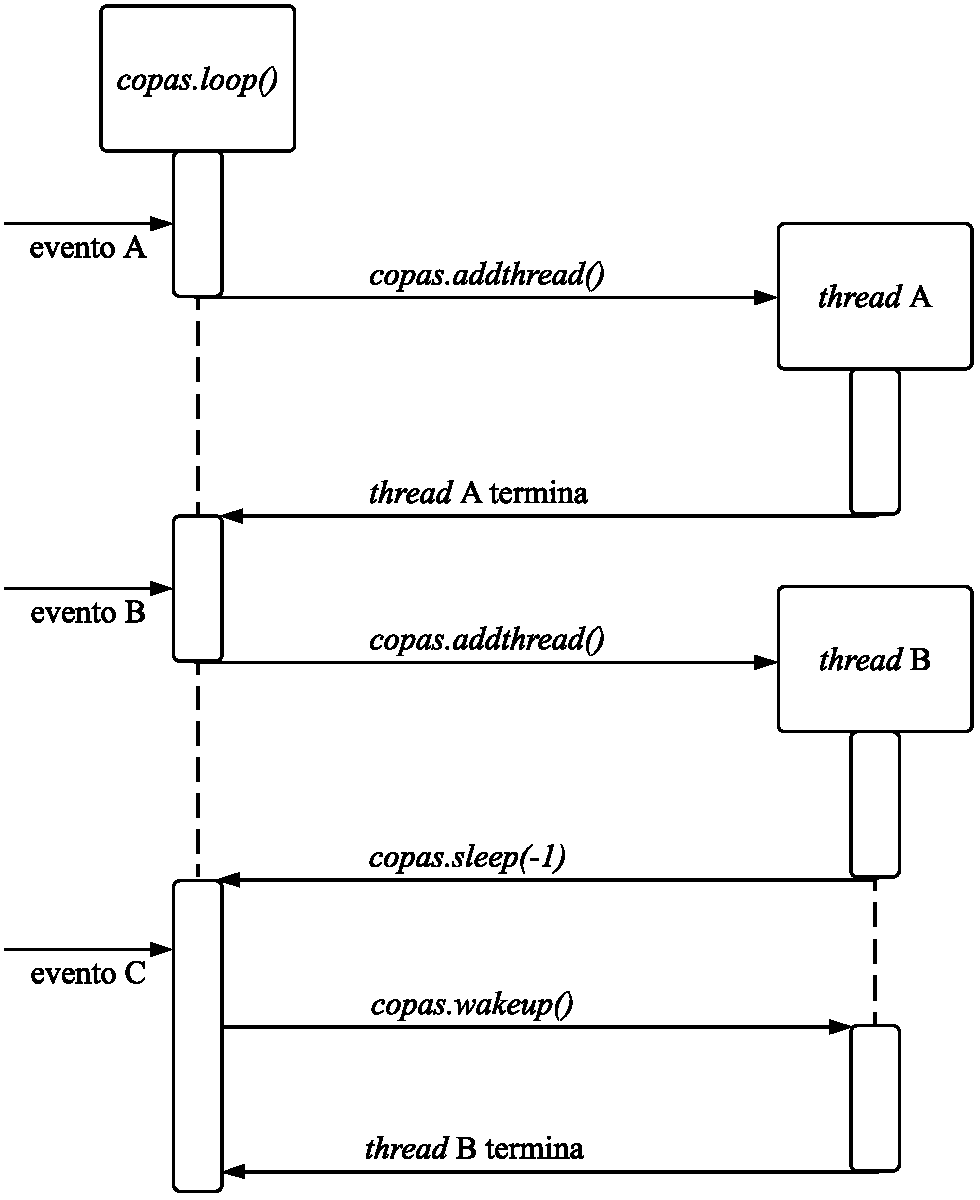
\includegraphics[width=0.8\textwidth]{./fig/events}
 \caption{Diagrama de sequência UML que modela a programação orientada a eventos utilizando a biblioteca Copas.}
 \label{fig:events}
\end{figure}

\section{Modelo de Concorrência}

O modelo de programação concorrente também foi necessário para atender aos requisitos de um cliente HTTP/2. Conforme visto na Seção \ref{subsec:fluxos}, um servidor pode multiplexar fluxos em uma única conexão HTTP/2. Isso significa que múltiplos fluxos podem estar sendo enviados pelo servidor de modo concorrente em qualquer momento durante uma conexão HTTP/2. Precisamos então de uma espécie de escalonador de fluxos para que possamos lidar com múltiplos fluxos sendo enviados concorrentemente por um servidor HTTP/2. 

Para recebermos e processarmos fluxos concorrentes, também precisamos de operações assíncronas ao nível de {\em sockets} TCP porque o modelo clássico de bloquear operações de rede não resolve o problema de tratar fluxos concorrentes na conexão TCP (que na verdade são apenas uma cadeia de bytes dentro do {\em buffer} TCP), além de ser uma abordagem ineficiente porque o cliente passaria a maior parte do tempo bloqueado na chamada de rede {\em receive} do {\em socket}.

Visando obter tanto concorrência para processar fluxos quanto operações de rede assíncronas, também utilizamos a biblioteca Copas. Nesse caso, o objetivo de Copas é escalonar múltiplos fluxos que podem estar presentes dentro da conexão TCP. As funcionalidades de Copas de prover operações assíncronas, descritas na Seção \ref{subsec:copas}, atendem bem o papel de escalonar os fluxos no nível de {\em sockets} TCP por combinar as características de {\em multithreading} cooperativa de Lua com as operações assíncronas de rede da biblioteca LuaSocket \cite{Nehab2007}.

Sempre que o {\em dispatcher} de Copas verifica que uma {\em thread} ainda está realizando alguma operação de rede {\em receive}, mas ainda não a concluiu, o {\em status} identificado por ``{\em timeout}'' de LuaSocket é sinalizado, o que significa que a operação retornou por incompleto. Nesse caso, a {\em thread} é suspensa por Copas. Internamente, o {\em dispatcher} de Copas implementa um {\em loop} despachante que emprega um mecanismo de notificação para obter o resultado do processamento de alguma operação de rede assíncrona contida em {\em threads} distintas, chamando uma por uma.

Assim, antes de detalharmos a implementação de ambos os modelos vistos e como eles foram empregados para implementar o lado cliente do HTTP/2, a Figura \ref{fig:deps} formaliza as dependências da biblioteca http2 através de um diagrama de componentes UML, em que cada biblioteca é representada por um componente. A biblioteca http2 depende da biblioteca LuaSocket para obter suporte tanto ao protocolo TCP quanto a funcionalidades de construção e processamento de URLs; de Copas para construirmos um escalonador de fluxos e obtermos operações de rede assíncronas e de LuaSec \cite{silvestre2018luasec} para fazer uso de conexões TLS seguras através do protocolo ALPN \cite{FriedlRFC7301}. Na próxima seção mostramos outro diagrama de componentes UML que ilustra a estrutura interna da biblioteca http2.

\begin{figure}[hbt!]
 \centering
  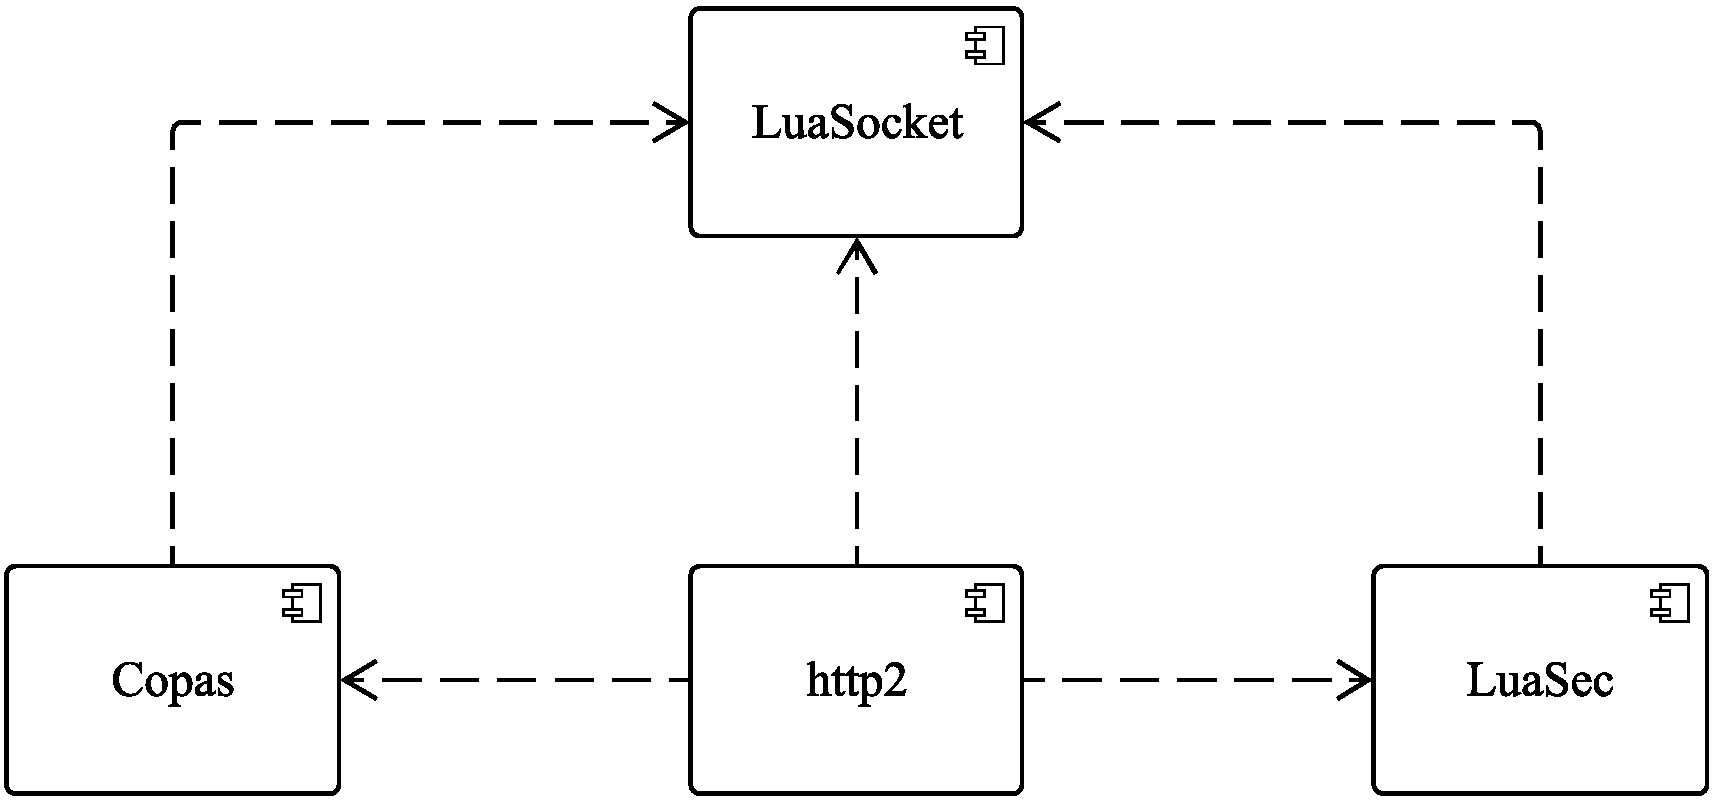
\includegraphics[width=\textwidth]{./fig/deps}
 \caption{Dependências da biblioteca http2 por outras bibliotecas de Lua.}
 \label{fig:deps}
\end{figure}

\section{Modelagem do Código-fonte}
\label{sec:components}

O diagrama de componentes UML retratado na Figura \ref{fig:deps} mostra como o código-fonte da biblioteca http2 foi modelado. O programador apenas interage com o módulo {\em http2} diretamente, sendo que os demais servem para oferecer interfaces projetadas especificamente em torno do suporte para as características de baixo nível do protocolo HTTP/2, além de permitir uma melhor organização de código através da modularização de funcionalidades.

\begin{itemize}
    \item {\em connection}: encapsula o gerenciamento de uma conexão HTTP/2.
    \item {\em stream}: encapsula o gerenciamento de fluxos HTTP/2.
    \item {\em framer}: realiza codificação e decodificação de quadros HTTP/2.
    \item {\em hpack}: realiza a codificação e decodificação de campos de cabeçalhos.
    \item {\em http2}: oferece a interface necessária para a criação de um cliente HTTP/2.
\end{itemize}

\begin{figure}[hbt!]
 \centering
  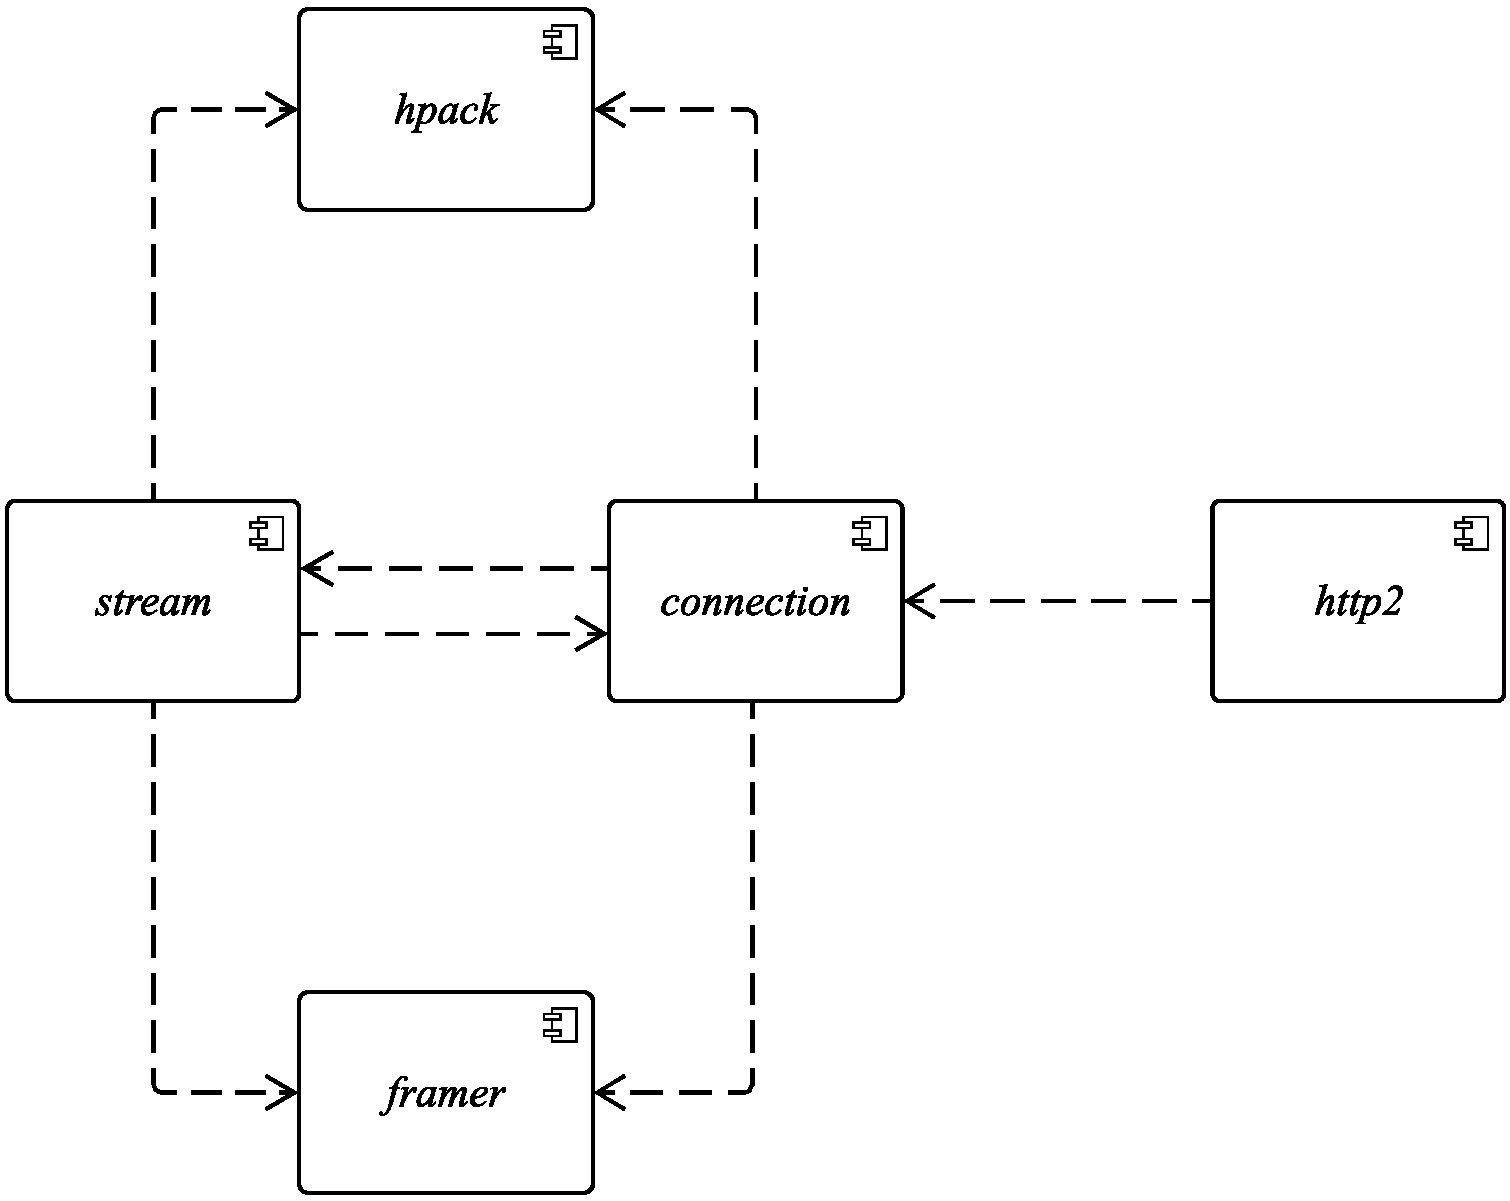
\includegraphics[width=\textwidth]{./fig/source}
 \caption{Componentes da biblioteca http2.}
 \label{fig:source}
\end{figure}

\subsection{Módulo {\em connection}}
\label{subsec:connection}

Alguns quadros HTTP/2 como {\em WINDOW\_UPDATE}, {\em SETTINGS} e {\em GOAWAY} são enviados a nível de uma conexão HTTP/2 e são pertinentes à toda sessão de comunicação entre clientes e servidores. No HTTP/2, é adotado a convenção de que esses quadros são enviados em um fluxo com identificador 0, indicando que esse fluxo é reservado para controlar a conexão e não pode ser utilizado para criar outros fluxos. Para tanto, o módulo {\em connection} foi criado para abstrair a responsabilidade de controlar uma conexão do módulo de fluxos {\em stream} (ver Seção \ref{subsec:stream}).

Essencialmente, o módulo {\em connection} oferece toda a lógica necessária para um cliente HTTP/2 se comportar com as exigências especificadas de um cliente HTTP/2 em termos do uso que ele faz da conexão HTTP/2 \footnote{Na verdade, esse comportamento é simétrico entre clientes e servidores, ou seja, as mesmas funcionalidades do módulo {\em connection} podem ser aplicadas tanto para clientes quanto para servidores HTTP/2.}. As funções disponibilizadas por esse módulo são:

\begin{itemize}
    \item \verb|connection:window_update(payload)|: envia um quadro {\em WINDOW\_UPDATE} com o seu respectivo corpo (\verb|payload|) para o servidor.
    \item \verb|connection:settings(payload)|: envia um quadro {\em SETTINGS} com o seu respectivo corpo (\verb|payload|) para o servidor.
    \item \verb|connection:goaway(payload)|: envia um quadro {\em GOAWAY} com o seu respectivo corpo (\verb|payload|) para o servidor.
    \item \verb|connection:parse_stream()|: encapsula toda a funcionalidade requerida para decodificar e processar um fluxo HTTP/2 contido no {\em buffer} do TCP.
    \item \verb|connection:new_stream(identifier)|: aloca e retorna um novo fluxo (\verb|stream|) para a conexão atual atribuindo-lhe o identificador \verb|identifier|.
    \item \verb|connection:new()|: construtor para uma nova conexão HTTP/2.
\end{itemize}

\subsection{Módulo {\em stream}}
\label{subsec:stream}

Uma única conexão HTTP/2 pode multiplexar múltiplos fluxos concorrentes: múltiplas requisições e respostas podem ser enviadas simultaneamente e os dados (quadros) do fluxo podem ser intercalados e priorizados. O módulo {\em stream} encapsula todo o gerenciamento de estados, transições, controle de fluxo e gerenciamento de erros no nível de fluxos conforme definidos pela especificação do HTTP/2. As funções disponibilizadas por esse módulo são:

\begin{itemize}
    \item \verb|stream:parse(frame)|: processa um quadro (\verb|frame|) proveniente de um fluxo HTTP/2.
    \item \verb|stream:headers(payload)|: envia um quadro {\em HEADERS} com o seu respectivo corpo (\verb|payload|) para o servidor.
    \item \verb|stream:window_update(payload)|: envia um quadro {\em WINDOW\_UPDATE} com o seu respectivo corpo (\verb|payload|) para o servidor.
    \item \verb|stream:new()|: construtor para um novo fluxo HTTP/2.
\end{itemize}

\subsection{Módulo {\em framer}}
\label{subsec:framer}

Como visto na Seção \ref{subsec:framing}, uma das melhorias trazidas pelo HTTP/2 em relação ao HTTP/1.1 é a forma como as mensagens HTTP são codificadas e decodificadas para serem enviadas na conexão TCP. No HTTP/2, cada mensagem HTTP/1 é mapeada para um quadro, a unidade de comunicação básica do HTTP/2, com o intuito de introduzir um novo enquadramento binário de mensagens. O módulo {\em framer} (``enquadrador'') implementa esse novo enquadramento, cuja função é descrever a maneira que quadros HTTP/2 são estruturados para serem formados em fluxos multiplexados. As funções auxiliares providas por esse módulo são:

\begin{itemize}
    \item \verb|encode(frame)|: gera um quadro HTTP/2 codificado em binário a partir de suas características desejáveis (cabeçalho e corpo) passadas como parâmetro (\verb|frame|).
    \item \verb|decode(buffer)|: decodifica um quadro HTTP/2 completo a partir de um \verb|buffer| TCP passado como parâmetro e retorna os campos referentes ao cabeçalho e ao corpo desse quadro.
\end{itemize}

\subsection{Módulo {\em hpack}}
\label{subsec:hpack}

A implementação do formato de compressão de cabeçalhos para o HTTP/2 (HPACK) \cite{BelsheRFC7541} para representar os cabeçalhos HTTP mais eficientemente é fornecido pelo módulo {\em hpack}. Apenas as funções utilitárias de codificação e decodificação de cabeçalhos foram implementadas nesse módulo, que são:

\begin{itemize}
    \item \verb|encode(header_list)|: responsável por codificar listas de pares chave-valor (\verb|header_list|) utilizando o algoritmo HPACK.
    \item \verb|decode(header_block)|: processa um bloco de cabeçalhos (\verb|header_block|).
    \item \verb|new(HEADER_TABLE_SIZE)|: cria e retorna um novo contexto HPACK a partir do parâmetro do quadro {\em SETTINGS}, \verb|HEADER_TABLE_SIZE|.
\end{itemize}

\begin{center}
 \begin{minipage}{0.7\textwidth}
  \begin{codigo}[H]
   \small
   \VerbatimInput[xleftmargin=10mm,numbers=left,obeytabs=true]{./prog/client.lua}
   \caption{\texttt{Cliente HTTP/2}}
   \label{code:client}
  \end{codigo}
 \end{minipage}
\end{center}

\subsection{Módulo {\em http2}}
\label{subsec:http2lua}

Talvez o módulo mais importante da implementação seja o {\em http2}, que merece atenção especial nesta seção. Trata-se de um módulo responsável por prover ao programador operações específicas de um cliente HTTP/2, bem como controlar o fluxo de execução do {\em loop} de eventos do Copas. Como o modelo de programação da biblioteca http2 é orientado a eventos, o código do programador é encarregado de tratar um evento emitido durante a sessão de comunicação com um servidor HTTP/2.

Para melhor expor o funcionamento desse módulo, considere um exemplo de um código cliente HTTP/2 que faz uso da biblioteca http2, ilustrado no Código \ref{code:client}. Nesse código, o programador registrou algumas funções anônimas atuando como funções de {\em callback} para tratarem de determinados eventos.

\begin{itemize}
    \item Na linha 5, uma função é registrada como tratadora do evento {\em on\_connect}, que é emitido quando uma conexão HTTP/2 com o servidor é estabelecida. Essa função de {\em callback} é invocada com o argumento \verb|session|, que representa uma sessão de comunicação HTTP/2 com o servidor.
    \item Na linha 6, uma requisição é submetida ao servidor conectado através da função \verb|request|. Essa requisição é realizada enviando cabeçalhos padrões definidos pela biblioteca, pois nenhum argumento foi passado para a função \verb|request|.
    \item Na linha 8, uma função é registrada como tratadora do evento {\em on\_response}, que é emitido quando um quadro {\em HEADERS} é recebido do servidor HTTP/2 conectado do fluxo correspondente à requisição \verb|req|. Essa função de {\em callback} é invocada com o argumento \verb|headers|, que contém o objeto que representa cabeçalhos HTTP/2 (uma tabela bidimensional de listas de cabeçalhos).
    \item Na linha 16, uma função é registrada como tratadora do evento {\em on\_data}, que é emitido quando o servidor HTTP/2 conectado termina de enviar dados (através de quadros {\em DATA}). Essa função de {\em callback} é invocada com o argumento \verb|data|, que é uma variável do tipo string contendo os dados transmitidos pelo servidor.
\end{itemize}

O Código \ref{code:client} pode ser facilmente estendido para realizar mais de uma requisição, bastando apenas repetir as chamadas de funções e trocando os nomes das variáveis associadas a requisição. Nesse contexto, o papel do módulo {\em http2} é abstrair o enquadramento de mensagens e multiplexação de fluxos de baixo nível realizados pela biblioteca, permitindo que o programador se concentre apenas na lógica de sua aplicação ou de seu cliente específico desde que as funções da API sejam corretamente chamadas.

As funções de alto nível fornecidas pelo módulo {\em http2} representam eventos que são emitidos quando computações específicas sobre dados transmitidos pelo servidor são enviados. Esses dados são passados como argumentos para as funções de {\em callback} registradas pelo programador para que ele possa tratá-los apropriadamente. Efetivamente, essas funções compõem a API da biblioteca http2 e são explicadas na Seção \ref{sec:api}. Uma função de baixo nível que faz parte da estrutura interna do módulo {\em http2} é chamada de {\em dispatcher} e é explicada em seguida.

\subsubsection{{\em Dispatcher}}

O {\em dispatcher} é uma função interna do módulo {\em http2} e é uma parte importante na biblioteca http2, pois ele é o responsável por realizar a tarefa de intercalar os quadros contidos em diferentes fluxos concorrentemente abertos em uma conexão TCP, bem como despachar {\em threads} associadas a esses fluxos. Ele foi construído baseando-se no modelo de programação concorrente com as características descritas nas Seções \ref{subsec:coroutines} e \ref{subsec:copas} e também no modelo de programação orientado a eventos com as características descritas no início deste capítulo.

Essencialmente, o {\em dispatcher} é um simples {\em loop} que recebe um quadro de um {\em buffer} TCP, determina a que fluxo esse quadro pertence e processa o seu conteúdo para que ele possa ser adequadamente intercalado. Como os fluxos HTTP/2 são concorrentes entre si, fica a cargo do {\em dispatcher} administrar esse nível de concorrência de modo a evitar problemas de coordenação e sincronização. Intercalado um quadro, o {\em dispatcher} verifica se alguma {\em thread} pode ser acordada em resposta ao término do processamento de determinados quadros de um fluxo.

É mais fácil entender o {\em dispatcher} visualizando seu código. O Código \ref{code:dispatcher} mostra como a implementação do {\em dispatcher} foi feita em função do gerenciamento de {\em threads} do Copas e do ciclo de vida um fluxo. Com o auxílio da função \verb|connection:parse_stream| (ver Seção \ref{sec:components}, intercalamos quadros HTTP/2 contidos em um fluxo específico. Através do {\em dispatcher}, o ciclo de vida de um fluxo (mostrado na Figura \ref{fig:ciclo_fluxo}) é efetivamente implementado. Observamos que esse ciclo de vida foi implementado utilizando o modelo de programação orientada a eventos: quando um determinado estado de um fluxo é alcançado, despachamos a {\em thread} (nesse caso, a {\em callback}) que trata desse estado com a função \verb|copas.wakeup|. O {\em loop} termina quando o estado {\em closed} é alcançado.

\section{API}
\label{sec:api}

A API da biblioteca http2 é definida em termos do modelo de programação orientada a eventos com as características descritas no início deste capítulo. O Código \ref{code:client} serve como um exemplo da maneira que o programador pode utilizar a biblioteca chamando funções da API disponibilizada. Todas as funções da API são definidas da seguinte forma:

\begin{itemize}
    \item \verb|http2.on_connect(url, callback)|: dispara a função de resposta \verb|callback| quando uma conexão HTTP/2 é estabelecida com o servidor identificado por \verb|url|. Retorna uma tabela representando uma sessão de comunicação HTTP/2.
    \item \verb|session.request([headers, body])|: submete uma requisição para o servidor HTTP/2 conectado na sessão \verb|session| e retorna uma tabela utilizada para invocar funções de {\em callback} associadas a essa requisição (vê-las a seguir). Caso estejam presentes, \verb|headers| é uma tabela bidimensional contendo listas de cabeçalhos HTTP/2 e \verb|body| é o corpo de uma requisição POST. Caso contrário, uma requisição GET é submetida com campos de cabeçalhos extraídos da URL passada como argumento da função \verb|on_connect|.
    \item \verb|req.on_response(callback)|: dispara a função de resposta \verb|callback| quando um quadro {\em HEADERS} é recebido do servidor HTTP/2 conectado do fluxo correspondente à requisição \verb|req|. A função \verb|callback| é invocada com uma tabela bidimensional contendo listas de cabeçalhos HTTP/2.
    \item \verb|req.on_data(callback)|: dispara a função de resposta \verb|callback| quando o servidor HTTP/2 conectado termina de enviar dados (através de quadros {\em DATA}). A função \verb|callback| é invocada com uma string contendo os valores dos dados recebidos.
\end{itemize}

\begin{center}
 \begin{minipage}{0.7\textwidth}
  \begin{codigo}[H]
   \small
   \VerbatimInput[xleftmargin=10mm,numbers=left,obeytabs=true]{./prog/dispatcher.lua}
   \caption{\texttt{Dispatcher}}
   \label{code:dispatcher}
  \end{codigo}
 \end{minipage}
\end{center}

\section{Considerações Finais}
\label{sec:implfinals}

O presente capítulo descreveu a implementação da biblioteca http2. O código-fonte, juntamente com o cliente mostrado na Seção \ref{fig:source} podem ser encontrados em \cite{Paulahttp2}. Requisições simples com os métodos de requisição {\em GET} e {\em POST} estão funcionando e foram testadas (outros métodos como {\em HEAD} e {\em PUT} podem ser simulados a partir desses dois), embora somente o HTTP/2 executado sobre uma conexão TLS seja suportado por padrão. Essa decisão foi tomada em reflexo da tendência atual de habilitar TLS por padrão tanto em navegadores quanto servidores e devido à pouca utilização do protocolo HTTP/2 sobre o TCP puro.

Como a implementação foi inteiramente escrita na linguagem Lua, alcançamos a capacidade de multiplataforma da biblioteca http2 porque Lua é uma linguagem multiplataforma. Com isso, a biblioteca segue a portabilidade de Lua. Uma restrição importante da implementação é que a biblioteca http2 não é compatível com versões anteriores à versão 5.3 de Lua. Essa decisão foi tomada sobretudo com base nas facilidades de manipulação de bits dessa versão e também visando a simplicidade da implementação.

Visto que o HTTP/2 é um protocolo extenso e complexo em funcionalidades, a biblioteca http2 oferece um suporte mínimo necessário para implementar as características básicas de um cliente HTTP/2. O programador não precisa ter total conhecimento do ciclo de vida de um fluxo porque atualmente apenas requisições simples podem ser feitas, ou seja, os estados e as transições que ocorrem na visão do programador são controlados internamente pela biblioteca. Na visão da biblioteca, contudo, implementamos os estados ocioso, aberto, semifechado (remoto) e fechado.

Como resultado, as principais características de um cliente HTTP/2 foram implementadas, como a habilidade de realizar multiplexação de fluxos e de fazer compressão e descompressão de campos de cabeçalhos. Em termos das outras novas características do HTTP/2, o {\em push} de requisições\slash respostas do servidor e priorizações de requisições não foram implementados, uma vez que o HTTP/2 não obriga o suporte para ambos esses mecanismos e também devido à limitação de tempo disponível para implementar essas novidades. Consequentemente, quadros {\em PRIORITY} e {\em PUSH\_PROMISE} não foram implementados. O quadro {\em PING} também não foi implementado porque ainda não mantemos verificações periódicas sobre o estado da conexão. Os outros quadros foram implementados e são suportados por padrão.
\chapter{Resultados Experimentais}
\label{cap:results}

Neste capítulo vamos apresentar alguns testes feitos para verificar o desempenho de um cliente escrito utilizando a biblioteca http2 quando submetido a diferentes fluxos de dados. Para efeito de análise, vamos utilizá-la para criar um cliente HTTP/2, chamado http2, a fim de compará-lo com outros clientes escritos em suas respectivas bibliotecas que também implementam o lado cliente do protocolo HTTP/2.

Os testes foram conduzidos da seguinte forma: selecionamos três clientes HTTP/2 populares para realizarem 10 requisições para um mesmo servidor HTTP/2 e para processarem as respostas enviadas por esse servidor simultaneamente na mesma conexão TCP. Essas 10 requisições serão feitas 10 vezes seguidas através de 10 diferentes execuções do cliente em particular. O servidor escolhido foi o servidor nghttpd da biblioteca nghttp2 (versão 1.30.0) \cite{nghttp2}. Os clientes escolhidos foram:

\begin{itemize}
    \item o cliente da biblioteca nghttp2 (versão 1.30.0): nghttp \cite{nghttp2}.
    \item um cliente que utiliza a biblioteca ``lua-http'' de Lua (versão 0.2) \cite{DaurminatorLuaHTTP}: lua-http.
    \item um cliente que utiliza a biblioteca ``http2'' de Node.js (versão 8.10.0) \cite{Nodejs}: nodejs.
\end{itemize}

O computador que hospedou o cliente HTTP/2 tem como especificações técnicas um processador Intel Core i3-4340 com 4 núcleos, cada um com 3.6 GHz; 6 GB de memória RAM; Ethernet 100 Mb/s e executa o sistema operacional GNU/Linux de 64 bits, {\em kernel} 4.4.0-17134-Microsoft. O computador que hospedou o servidor HTTP/2 tem como especificações técnicas um processador AMD Dual Core E1-500 com 2 núcleos, cada um com 1.48 GHz; 4 GB de memória RAM; Ethernet 100 Mb/s e  executa o sistema operacional GNU/Linux de 64 bits, {\em kernel} 4.15.0-38-generic.

Tentamos diversificar a escolha dos clientes de modo a testarmos como diferentes métodos para implementá-los podem impactar em seus desempenhos nos cenários de teste deste trabalho. O cliente nghttp foi escolhido por ter sido implementado na linguagem compilada C, na qual a expectativa é que ele obtenha um desempenho superior em relação aos demais, que são implementados em linguagens de {\em scripting}. O cliente lua-http foi selecionado por se assemelhar com o cliente http2 em termos da linguagem Lua, apesar de ambos empregarem diferentes mecanismos de implementação. O cliente nodejs foi escolhido por também ter sido implementado em uma linguagem de {\em scripting}.

Durante a execução dos testes, conectamos o computador cliente e o computador servidor na mesma rede LAN, bem como suspendemos quaisquer intervenções externas da rede que possam impactar negativamente a vazão de dados nos enlaces Ethernet. Apesar de estudos como \cite{Saxce7179400, Oda8319285} mostrarem que o HTTP/2 apenas traz vantagens em certas condições de rede, é importante conduzir testes para comparar o desempenho da implementação do cliente http2 com outros clientes HTTP/2 quando múltiplas requisições simultâneas são feitas na mesma conexão TCP, ao mesmo tempo evitando uma fuga ao escopo deste trabalho.

Nas Figuras \ref{fig:1,5MB}, \ref{fig:10MB} e \ref{fig:100MB}, medimos o tempo médio de execução de três testes feitos como descritos a seguir. Em cada teste, realizamos 10 execuções de cada cliente, cada execução submetendo um total de 10 requisições simultâneas na mesma conexão TCP (e não sequenciais ou em diferentes conexões TCP para cada requisição, como no HTTP/1.1) para o servidor.

O primeiro retrata melhor o cenário atual de uma requisição por uma página Web de tamanho típico de 1,5 megabytes \cite{HTTPArchive}. Pelos resultados mostrados na Figura \ref{fig:1,5MB}, observamos que o cliente da biblioteca http2 se sobressaiu no cenário de uma curta troca de dados e, nesse caso, com tempo de 1,08 segundos para baixar 1 megabyte. Em comparação, para baixar 1 megabyte, o cliente lua-http precisou de 1,13 segundos; o cliente nodejs, 1,38 segundos e o nghttp, 1,1 segundos.

O segundo teste fez com que os clientes realizassem requisições para um arquivo de 10 MB. Pelos registros resumidos na Figura \ref{fig:10MB}, o cliente http2 em questão ainda mostra uma boa vazão ao levar 1,11 segundos para baixar 1 megabyte nessa situação de um médio fluxo de dados. Em comparação, para baixar 1 megabyte, o cliente lua-http precisou de 1,13 segundos; o cliente nodejs, 1,17 segundos e o cliente nghttp, 1,10 segundos.

No último teste, os clientes submeteram requisições para um arquivo de 100 MB. Depois, medimos o tempo médio de execução (em segundos) e obtivemos o satisfatório resultado de que o cliente http2 teve um tempo comparável com cliente nghttp. Em média, para baixar 1 megabyte nesse cenário, o cliente http2 levou 0,89 segundos. Em comparação, para baixar 1 megabyte, o cliente lua-http precisou de 0,94 segundos; o cliente nodejs, 0,89 segundos e o cliente nghttp, também 0,89 segundos.

É importante observar que o cliente http2 foi implementado visando funcionalidades mínimas necessárias para um cliente HTTP/2, pois ela somente cumpre com os requisitos mínimos do protocolo HTTP/2. Em contrapartida, as outras implementações, por serem mais maduras, podem ter uma lógica de processamento mais bem elaborada internamente, podendo impactar mais na vazão dos dados transmitidos pelo servidor.

\begin{figure}[hbt!]
 \centering
  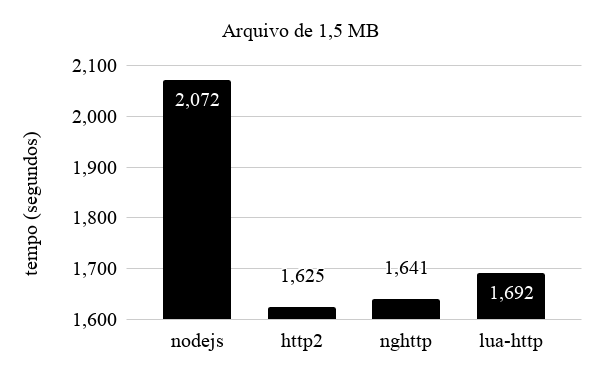
\includegraphics[width=0.65\textwidth]{./fig/1,5MB}
 \caption{Tempo médio de execução de quatro clientes HTTP/2, onde cada um fez 10 requisições de um arquivo de 1,5 megabytes.}
 \label{fig:1,5MB}
\end{figure}

\begin{figure}[hbt!]
 \centering
  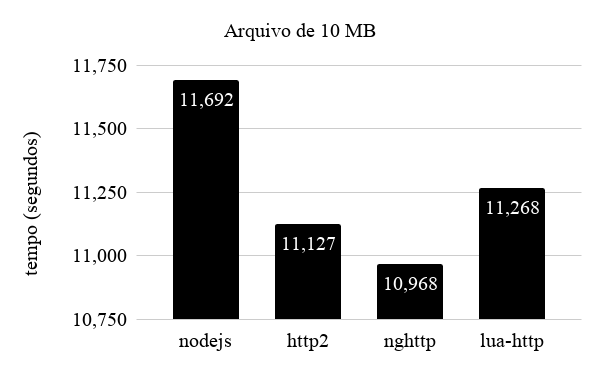
\includegraphics[width=0.65\textwidth]{./fig/10MB}
 \caption{Tempo médio de execução de quatro clientes HTTP/2, onde cada um fez 10 requisições de um arquivo de 10 megabytes.}
 \label{fig:10MB}
\end{figure}

\begin{figure}[hbt!]
 \centering
  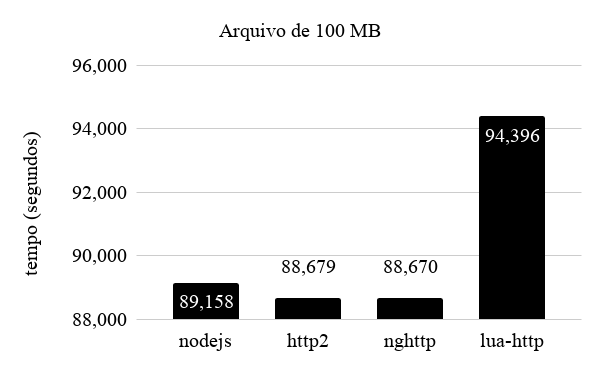
\includegraphics[width=0.65\textwidth]{./fig/100MB}
 \caption{Tempo médio de execução de quatro clientes HTTP/2, onde cada um fez 10 requisições de um arquivo de 100 megabytes.}
 \label{fig:100MB}
\end{figure}
\chapter{Considerações Finais}
\label{cap:conclusion}

Este trabalho apresentou as características teóricas e práticas da implementação de uma biblioteca cliente HTTP/2 multiplataforma em Lua, denominada http2. A metodologia empregada para desenvolver a biblioteca http2 com a característica de ser multiplataforma tem por base o modelo de programação orientado a eventos o modelo de programação concorrente de Lua. O modelo orientado a eventos foi adotado para implementar os estados de um fluxo HTTP/2, bem como para fornecer uma API baseada em {\em callbacks}. O modelo concorrente permitiu que fluxos HTTP/2 multiplexados pudessem ser recebidos e processados de forma concorrente e assíncrona.

A programação de clientes HTTP/2 é permitida através da presente biblioteca, que é multiplataforma por ser escrita inteiramente em Lua, oferecendo aos programadores uma simples API para realizarem requisições HTTP/2 simultâneas na mesma conexão TCP, aproveitando os benefícios de desempenho trazidos pelo protocolo HTTP/2. A construção de clientes HTTP/2 e de aplicações Web que executam sobre o HTTP/2 é amplamente encorajada, principalmente devido as vantagens de desempenho em relação ao HTTP/1.1.

No entanto, o HTTP/2 é um protocolo complexo. É difícil implementar o lado cliente desse protocolo com todas as suas características em escala de produção. Com ciência disso, decidimos implementar apenas as funcionalidades essenciais que permitem a criação de clientes HTTP/2 em conformidade com a especificação do HTTP/2, incluindo as duas principais características do HTTP/2: a capacidade de realizar múltiplas requisições simultâneas na mesma conexão TCP e de realizar a compressão de campos de cabeçalhos utilizando o HPACK.

Em termos do suporte às características do HTTP/2: permitimos multiplexação de fluxos na mesma conexão TCP; implementamos o algoritmo de compressão de campos de cabeçalhos do HTTP/2, o HPACK; implementamos os quadros {\em DATA}, {\em HEADERS}, {\em RST\_STREAM}, {\em SETTINGS}, {\em GOAWAY}, {\em WINDOW\_UPDATE} e {\em CONTINUATION}; implementamos os estados de um fluxo ocioso, aberto, semifechado (remoto) e fechado; requisições {\em GET} e {\em POST} triviais foram implementadas, possibilitando que outros métodos de requisições que são derivados desses dois (como {\em HEAD} e {\em PUT}) sejam utilizados.

\section{Trabalhos Futuros}
\label{sec:futurework}

Uma primeira proposta para trabalhos futuros é a implementação das características de um cliente HTTP/2 que não foram implementadas neste projeto. Priorização de requisições podem trazer benefícios de desempenho para a aplicação quando vários fluxos são abertos. {\em Push} de requisição\slash resposta do servidor podem ser implementados e aceitos quando um servidor solicita esse mecanismo, podendo melhorar significativamente o desempenho da aplicação dependendo da política de {\em push} do servidor.

Como o protocolo HTTP/2 não alterou a semântica existente do HTTP/1.1, seria interessante dar suporte a mais características especificadas do HTTP/1.1, como {\em lookups} DNS e gerenciamento de {\em cookies}.

Uma outra forma de melhorar a implementação seria adicionando mais tratamentos de erros e, consequentemente, melhorando a conformidade de clientes escritos utilizando a biblioteca http2 com os tratamentos de erros do HTTP/2.

Por outro lado, mudanças feitas nesses sentidos precisam ser feitas de forma transparente com o código do programador, ajustando a API para que as mudanças internas sejam refletidas externamente na utilização da biblioteca.

Outra abordagem mais avançada seria reavaliar a forma de funcionamento da biblioteca Copas, levando em consideração que ela possui um único {\em loop} de estado global. Seria interessante alterar Copas para, por exemplo, não dependermos de um único {\em loop} global, de forma que possamos controlar mais facilmente a programação de clientes HTTP/2.

%------------------------------------------------------------ BIBLIOGRAFIA %
\cleardoublepage
%\nocite{*} %%% Retire esta linha para gerar a bibliografia com apenas as
           %%% referências usadas no seu texto!
\arial
\bibliographystyle{unsrt}
\bibliography{./bib/http2} %%% Nomes dos seus arquivos .bib
\label{ref-bib}

%--------------------------------------------------------------- APÊNDICES %
\end{document}

%------------------------------------------------------------------------- %
%        F I M   D O  A R Q U I V O :  m o d e l o - t e s e . t e x       %
%------------------------------------------------------------------------- %
